%!TEX root=./LIVRO.tex

\chapter{Gêneros textuais argumentativos}
\markboth{Módulo 1}{}

\section{Habilidades do SAEB}

\begin{itemize}
\tightlist
\item
  Identificar o uso de recursos persuasivos em textos verbais e não
  verbais.
\item
  Identificar teses, opiniões, posicionamentos explícitos e argumentos
  em textos.
\end{itemize}

\subsection{Habilidade da BNCC}

\begin{itemize}
\tightlist
\item
  EF89LP04.
\end{itemize}

\conteudo{Argumentar é convencer, persuadir o outro de que os argumentos usados
têm procedência lógica e podem ser comprovados.

Os gêneros textuais argumentativos têm o objetivo de apresentar e
defender um ponto de vista sobre um assunto por meio de argumentação e
recursos persuasivos que buscam a adesão do interlocutor. Duas
características fundamentais dos textos argumentativos são a emissão de
juízo de valor e o emprego de argumentos e recursos persuasivos para
justificar o ponto de vista.

Entre esses gêneros, destacam-se o \textbf{artigo de opinião}, a
\textbf{resenha crítica}, a \textbf{carta de leitor},
o~\textbf{editorial} e o \textbf{anúncio publicitário}.}

\begin{itemize}
\tightlist
\item
  O artigo de opinião tem o objetivo de opinar sobre um assunto
  relevante que esteja em evidência na sociedade. Seu público-alvo são
  os leitores de um jornal, revista ou portal de notícias. A linguagem
  pode ter tom mais impessoal (em 3ª pessoa) ou pessoal (em 1ª pessoa),
  e o nível de formalidade pode variar conforme o perfil do público.
\item
  A resenha crítica tem o objetivo de apresentar um resumo comentado e
  opinativo sobre um filme, uma série, um livro ou outra obra, de modo a
  persuadir o leitor a consumir ou não aquela produção. Seu público-alvo
  são os fãs ou interessados em consumir o filme, a série, o livro ou
  outra obra. A linguagem pode ser coloquial e pode ter tom mais
  impessoal (em 3ª pessoa) ou pessoal (em 1ª pessoa); o nível de
  formalidade pode variar
\item
  A carta de leitor tem o objetivo de expor ponto de vista acerca de
  determinado assunto publicado em um jornal ou uma revista. Seu
  público-alvo é o editor da revista ou do jornal, ou o autor da matéria
  jornalística que motivou a carta de leitor. A linguagem pode ter tom
  mais impessoal (1ª pessoa) ou pessoal (em 1ª pessoa).
\item
  O editorial tem o objetivo de expor a opinião do jornal ou da revista
  sobre assuntos abordados nas notícias e reportagens publicados naquele
  veículo de informação. Seu público-alvo são os leitores daquele jornal
  ou revista. A linguagem, geralmente, tem tom impessoal (3ª pessoa),
  por representar a opinião da equipe jornalística, e não de uma pessoa.
\item
  O anúncio publicitário tem o objetivo de vender um produto ou divulgar
  uma ideia. Seu público-alvo pode ser geral ou específico, dependendo
  do produto ou da ideia. A linguagem é variada e pode valer-se de texto
  verbal e texto não verbal.
\end{itemize}

\section{Atividades}

\num{1} Numere a segunda coluna de acordo com a primeira considerando o
teor dos argumentos que você espera encontrar em cada gênero textual
argumentativo listado.

\begin{multicols}{2}
I. Artigo de opinião


II. Anúncio publicitário


III. Resenha crítica 
\columnbreak

(~\rosa{III} ) Qualidade dos personagens, do
enredo, da narrativa, do desfecho, da trilha sonora etc. 

(~\rosa{I} ) Dados e estatísticas, citação de
especialista na área, exemplificação de fatos importantes e de
repercussão etc.

(~\rosa{II}) Imagem de
personalidade famosa, pergunta provocativa, trocadilhos, apelo ao
consumo etc.
\end{multicols}

\num{2} Associe as duas colunas de acordo com o tipo de argumento
exemplificado em cada parágrafo.

\begin{multicols}{2}
I. Alusão histórica 

II. Exemplificação

III. Autoridade

IV. Factual
\columnbreak

(~\rosa{IV}~) A internet é uma tecnologia que faz
parte do cotidiano das pessoas e que protagoniza a cultura
contemporânea. Ela é uma ferramenta que encurta distâncias e confere um
caráter de acessibilidade universal à informação e aos mais diversos
campos do conhecimento humano, sendo um dos principais agentes da
globalização 

(~\rosa{III}~) Em primeiro lugar,
deve-se ressaltar a ausência de medidas governamentais para combater a
venda de dados pessoais e a manipulação do comportamento nas redes.
Segundo o pensador Thomas Hobbes, o Estado é responsável por garantir o
bem-estar da população, entretanto, isso não ocorre no Brasil.

(~\rosa{I}~) A utilização dos meios de comunicação para
manipular comportamentos não é recente no Brasil: ainda em 1937, Getúlio
Vargas apropriou-se da divulgação de uma falsa ameaça comunista para
legitimar a implantação de um governo ditatorial. 

(~\rosa{II}~) Em consequência disso, os deficientes auditivos
encontram inúmeras dificuldades em variados âmbitos de suas vidas. Um
exemplo disso é a difícil inserção dos surdos no mercado de trabalho,
devido à precária educação recebida por eles e ao preconceito intrínseco
à sociedade brasileira.
\end{multicols}

\num{3} Você leu uma matéria num jornal e discordou do posicionamento do
jornalista ao abordar o tema. Você, então, decide interagir com o jornal
e com o público que o acompanha, emitindo sua opinião sobre o assunto
publicado naquela edição do jornal e questionando a abordagem do
redator. Marque o gênero textual que você deverá produzir para concluir
seu objetivo.

\begin{boxlist}
\boxitem{\white{X}} Artigo de opinião
\boxitem{X} Resenha crítica
\boxitem{\white{X}} Carta de leitor
\end{boxlist}

\num{4} Você foi convidado a escrever um texto opinativo sobre uma série
de televisão de sua preferência para o jornal da escola e fazer a
indicação dessa obra para os alunos como forma de enriquecer seu
conhecimento cultural. Assinale o gênero textual que você precisará
escrever para realizar essa tarefa.

\begin{boxlist}
\boxitem{\white{X} } Artigo de opinião
\boxitem{X} Resenha crítica
\boxitem{\white{X}} Carta de leitor
\end{boxlist}

\num{5} Escreva um texto opinativo sobre um livro, um filme ou uma série
que você conheça para ser publicado no jornal da escola e faça a
indicação da obra para os alunos. Procure apresentar argumentos
plausíveis para convencê-los de que vale a pena conhecê-la.

\linhas{15}
% \coment{A atividade se destina a colocar em prática a teoria básica estudada sobre o gênero argumentativo resenha crítica. Talvez esse gênero textual já tenha sido estudado mais a fundo e de forma sistematizada; entretanto, mais importante do que atender às exigências da teoria de construção composicional, conteúdo temático e estilo do gênero é o aluno entender que precisa convencer seu leitor com uma avaliação convincente da obra, por meio de argumentos que convençam o leitor a se interessar por conhecê-la.}

Leia o texto para resolver as atividades de 6 a 10.

\begin{figure}
\centering

\includegraphics[width=4.21103in,height=3.86458in]{./imgSAEB_8_POR/media/image41.png}
\end{figure}

\num{6} Esse cartaz é um texto argumentativo. Nele, os recursos
persuasivos são construídos por meio da associação entre texto verbal e
texto não verbal. Cite o recurso não verbal que foi utilizado para
convencer o leitor a adotar o comportamento explicitado no texto verbal.

\reduline{O recurso persuasivo não verbal utilizado para se obter a adesão do leitor é a imagem de duas mãos que acolhem uma gota de água que cai, num gesto de proteção com esse recurso.\hfill}
\linhas{5}

\num{7} Qual é a ideia representada pela ilustração presente no cartaz?

\reduline{A figura da torneira aberta representa a ideia de cuidado com a água.\hfill}
\linhas{2}

\num{8} De que modo as cores predominantes no cartaz relacionam-se com o
tema central dele?

\reduline{O predomínio de azul relaciona-se à água, o bem que está sendo celebrado no cartaz, assim como a outra cor predominante (verde) relaciona-se com o cuidado com o meio ambiente.\hfill}
\linhas{6}

\num{9} Qual é o sentido global que se constrói a partir da associação
entre o texto verbal e o texto não verbal do cartaz?

\reduline{No cartaz, está ilustrada uma situação de cuidado e proteção com a água, o que se reflete na ideia de economia de água traduzida no texto verbal.\hfill}
\linhas{6}

\num{10} Justifique importância da publicação desse cartaz para a
conscientização da população.

\reduline{Uma possibilidade de resposta é que
a publicação desse cartaz transmite a mensagem da preservação da água de
forma simples e corriqueira, pelo fato de usar frases pouco complexas e
ilustrações facilmente reconhecíveis pela população em geral.\hfill}
\linhas{6}

\section{Treino}

\textbf{Leia o texto para responder às questões 1 e 2.}

\begin{quote}
\textbf{A família Mandible - Lionel Shriver}
\end{quote}

\begin{quote}
Se você me acompanha, sabe que sou fascinada por distopias. Não perco a
oportunidade de ler uma boa história desse gênero. Então, quando recebi
o livro ``A família Mandible'' como a escolha de janeiro do Clube
Intrínsecos, número 028, percebi que se tratava de uma sátira distópica.
Minha curiosidade ficou imensa e eu mal podia esperar para devorar o
livro assim que tivesse a chance. Fiquei ainda mais intrigada quando
descobri que, em vez de abordar uma distopia futurista com invasões de
zumbis ou alienígenas, o enredo tratava de um apocalipse financeiro que
levou os Estados Unidos da América, uma das maiores potências mundiais,
ao colapso. No entanto, será que, ao final da leitura, achei que toda
essa curiosidade valeu a pena? Venha descobrir!
\end{quote}

\fonte{Fonte de pesquisa: Evelyn Butgnoli. Viagem
literária. A família Mandible - Lionel Shriver. Disponível em: \url{http://www.viagemliteraria.com.br/2021/03/a-familia-mandible-lionel-shriver.html.Acesso em: 10 fev. 2023.}}

\num{1} Os gêneros textuais podem ser reconhecidos com base em
determinadas características que apresentam. Considerando-se as
características do texto lido, ele corresponde ao gênero

\begin{escolha}
\item
  crônica, porque a resenhista faz uma narração do seu cotidiano como
  leitora.
\item
  diário, porque a resenhista conta suas experiências literárias em um
  dia específico.
\item
  resenha crítica, porque a resenhista apresenta sua avaliação sobre um
  livro que leu.
\item
  anúncio publicitário, porque a resenhista elogia um livro para
  convencer o leitor a comprá-lo.
\end{escolha}

\num{2} A autora ressalta um diferencial do livro. Esse diferencial,
segundo ela, foi o que a convenceu a lê-lo e também pode interessar ao
público. O diferencial está descrito em:

\begin{escolha}
\item ``Venha descobrir!''

\item ``Se você me acompanha, sabe que sou fascinada por distopias.''

\item ``No entanto, será que, ao final da leitura, achei que toda essa
curiosidade valeu a pena?''

\item ``em vez de abordar uma distopia futurista com invasões de zumbis ou
alienígenas, o enredo tratava de um apocalipse financeiro''.
\end{escolha}

\num{3} Leia o cartaz.

\begin{figure}
\centering

\includegraphics[width=4.21103in,height=2.86458in]{./imgSAEB_8_POR/media/image40.png}
\end{figure}

A importância da figura sorridente do personagem Zé Gotinha deve-se ao
fato de que

\begin{escolha}
\tightlist
\item
  o personagem é o exemplo ruim de alguém que se vacina.
\item
  a intenção da campanha é motivar as crianças a se vacinarem.
\item
  a campanha pretende criar a ideia de que a vacina afasta a felicidade.
\item
  as doenças contra as quais se anuncia são leves e não causam grandes
  problemas.
\end{escolha}

\begin{escolha}
\tightlist
\item
  Incorreta. O objetivo do personagem é justamente o de aproximar a
  vacinação das crianças.
\item
  Correta. A felicidade do personagem mostra como se vacinar é algo bom.
\item
  Incorreta. A ideia é justamente o contrário, já que a campanha serve
  para mostrar que a vacinação é algo bom.
\item
  Incorreta. As doenças são graves, e a vacinação é importante, mas a
  felicidade do personagem não diminui esses dados.
\end{escolha}

\chapter{Gêneros textuais informativos}
\markboth{Módulo 2}{}

\section{Habilidades do SAEB} 

\begin{itemize}
\item Identificar elementos constitutivos de textos pertencentes ao domínio jornalístico/midiático.
\item Identificar formas de organização de textos normativos, legais e/ou reinvindicatórios.
\item Identificar elementos constitutivos de gêneros de divulgação científica.
\item Analisar a relação temática entre diferentes gêneros jornalísticos.
\end{itemize}

\subsection{Habilidades da BNCC}

\begin{itemize}
\tightlist
\item
  EF69LP02, EF69LP20, EF69LP27, EF08LP01.
\end{itemize}

\conteudo{Os gêneros textuais informativos têm o objetivo de informar sobre
determinado assunto, objeto ou fato. Por isso, são centrados na
informação a ser transmitida, sem juízo de valor por parte do autor,
prezando assim pela isenção e pela imparcialidade, diferentemente do que
ocorre nos gêneros argumentativos, que são opinativos. Entre os gêneros
informativos, destacam-se a \textbf{notícia}, a \textbf{reportagem}, o
\textbf{artigo científico} e o \textbf{verbete}.

Por não conterem opinião ou pontos de vista do autor, não pretendem
também convencer o leitor ou ganhar sua adesão. Sendo assim, não há
margem para interpretações duplas; pelo contrário, a compreensão do
conteúdo pelo leitor é restrita aos limites do texto propriamente dito.

A linguagem nos gêneros textuais informativos é objetiva (impessoal, em
3ª pessoa), concisa (focada nas informações essenciais), denotativa
(literal) e clara (precisa), com predominância da norma-padrão.

Pode haver nos gêneros textuais informativos o uso de dados,
estatísticas e citação para reforçar a veracidade da informação e
garantir a credibilidade dela, já que se trata do domínio jornalístico e
do científico, que têm seu rigor e compromisso próprios.}

\section{Atividades}

Para resolver as atividades de 1 a 4, leia uma manchete e o respectivo
subtítulo a seguir.

\begin{quote}
\textbf{Estudo confirma que o vírus da zika não é transmitido pela
saliva} 
\emph{Baixas quantidades virais, substâncias antimicrobianas
naturais e textura viscosa dificultam a infecção do zika por meio de
contato com a saliva, de acordo com o artigo.}
\end{quote}

\fonte{G1. Estudo confirma que o vírus da zika não é transmitido pela saliva. Disponível em: \url{https://g1.globo.com/bemestar/zika-virus/noticia/estudo-confirma-que-o-virus-da-zika-nao-e-transmitido-pela-saliva.ghtml. Acesso em: 16 maio 2023.}}

\num{1} Apenas com base nessas informações, provavelmente você logo
reconheceu o gênero textual a que o texto pertence e deduziu o objetivo
comunicativo dele. Cite-os.

\reduline{Trata-se de uma notícia, e o objetivo comunicativo é informar sobre uma descoberta científica que envolve o vírus da zika e sua transmissão.\hfill}
\linhas{4}

\num{2} Aponte e explique uma marca de impessoalidade e objetividade
presente nesse texto.

\reduline{No texto, isso é feito por meio do uso da 3ª pessoa e da ausência de adjetivação valorativa.\hfill}
\linhas{3}

\num{3} Qual recurso é utilizado no texto para afastar a
responsabilidade pelo que é dito?

\reduline{Trata-se da citação de um estudo científico prévio que pesquisou e fez conclusões sobre o tema.\hfill}
\linhas{4}

\num{4} Há mais de uma interpretação possível para o conteúdo desse
texto? Justifique sua resposta.

\reduline{Não. Há apenas uma interpretação possível porque o texto privilegia o
sentido literal das palavras, dando ao leitor pouca possibilidade de
interpretação para além do sentido pretendido, já que as palavras são
empregadas em seu sentido original, dicionarizado.\hfill}
\linhas{6}

Para resolver as atividades 5 e 6, leia o texto a seguir.

\begin{quote}
\textbf{Nova espécie de orangotango descoberta em pequena ilha}
\end{quote}

\begin{quote}
Cientistas da universidade suíça de Zurique que estão trabalhando em
Sumatra, uma ilha na Indonésia, conseguiram confirmar que uma pequena
população de orangotangos é, de fato, uma espécie nova e anteriormente
desconhecida.
\end{quote}

\begin{quote}
A investigação teve início em 2013, quando os restos mortais de um
orangotango macho revelaram que certas características dentárias e
cranianas do primata eram distintas e exclusivas, conforme informado
pela instituição acadêmica.
\end{quote}

 \fonte{Fonte de pesquisa: Vix. Mulher. Nova espécie de
orangotango descoberta em pequena ilha: como são os tapanuli?.
Disponível em: \url{https://www.mulher.com.br/atualidades/ciencia/nova-especie-de-orangotango-descoberta-em-pequena-ilha-como-sao-os-tapanuli}.
Acesso em: 16 fev. 2023.}

\num{5} Sobre o texto, responda às perguntas básicas de estruturação de
uma notícia.

a) O fato. O que aconteceu? 

  \reduline{Descoberta de uma nova espécie de orangotango\hfill}
  \linhas{2}

b) O modo. De que forma aconteceu? 

    \reduline{Pela análise das características dos dentes e do crânio de um orangotango macho morto.\hfill}
    \linhas{2}

c) O local. Onde aconteceu? 

  \reduline{Na pequena ilha de Sumatra.\hfill}
  \linhas{2}

d) O tempo. Quando aconteceu? 

  \reduline{Em 2013.\hfill}
  \linhas{2}

e) Os participantes. Quem são as pessoas envolvidas? 

  \reduline{Pesquisadores da universidade suíça de Zurique.\hfill}
  \linhas{2}

\num{6} Assinale com um X as características que você identifica no
texto, de acordo com o gênero textual a que ele pertence.

\begin{boxlist}
\boxitem {X} Objetividade (3ª pessoa). 
\boxitem {X} Impessoalidade.
\boxitem {X} Citação de autoridade no assunto. 
\boxitem {\white{X}} Parcialidade. 
\boxitem {X} Concisão (foco nas informações essenciais). 
\boxitem {X} Escrita em norma-padrão. 
\boxitem {\white{X}} Prolixidade.
\boxitem {\white{X}} Sentido conotativo (figurado).
\boxitem {\white{X}} Escrita em norma não padrão. 
\boxitem {X}
Imparcialidade.
\boxitem {X} Sentido denotativo (literal).
\boxitem {\white{X}} Pessoalidade.
\boxitem {\white{X}} Subjetividade (1ª pessoa).
\end{boxlist}

Para resolver as atividades de 7 a 10, leia o texto a seguir.

\begin{quote}
\textbf{Plantas medicinais: uma abordagem sobre o uso seguro e racional}
\end{quote}

\begin{quote}
Diversas espécies vegetais possuem propriedades medicinais e servem como
complementos terapêuticos no tratamento de doenças, trazendo benefícios
consideráveis para a saúde quando utilizadas de forma racional e
apropriada. No entanto, as plantas contêm uma ampla gama de compostos
químicos, que podem ser benéficos, mas também acarretar potenciais
riscos à saúde. Portanto, é crucial que os usuários, profissionais da
área da saúde e prescritores possuam conhecimento sobre as plantas,
incluindo sua identificação correta, conservação, métodos de preparo e
uso, bem como os possíveis efeitos colaterais.
\end{quote}

\begin{quote}
Neste artigo, são abordadas as plantas medicinais, seus riscos e
benefícios, levando em consideração as publicações científicas
contemporâneas. Destaca-se a importância dos profissionais de saúde como
educadores e promotores de saúde nas comunidades, especialmente aquelas
que utilizam o Sistema Único de Saúde.
\end{quote}

\fonte{Fonte de pesquisa: SCIELO. Plantas medicinais: uma abordagem sobre o uso seguro e racional. Disponível em: \url{https://www.scielo.br/j/physis/a/kwsS5zBL84b5w9LrMrCjy5d/. Acesso em: 18 fev. 2023.}}

\num{7} O texto relaciona-se ao gênero artigo. Marque o subgênero a que
ele se relaciona.

\begin{boxlist}
\boxitem{X} Artigo científico.
\boxitem{\white{X}} Artigo de opinião.
\end{boxlist}

\num{8} Qual elemento ou característica do texto determinou sua resposta
à questão anterior?

\reduline{Uma possibilidade de resposta é a ausência de valoração e
juízo de valor no artigo científico e a centralidade no objetivo
comunicativo de informar.}
\linhas{6}

\num{9} O que o trecho ``levando em consideração as publicações
científicas contemporâneas'' revela sobre o conteúdo do texto? Explique.

\reduline{O trecho é uma representação de autoridade no assunto em questão. Não há
citação explícita, mas fica claro que o conteúdo do artigo se apoiará em
comprovações científicas prévias que já abordaram o assunto. Ou seja,
parte do conteúdo do artigo já foi dita ou afirmada por outrem.}
\linhas{6}

\num{10} Em sua opinião, esse artigo é voltado para leitores comuns ou
para leitores específicos? Justifique sua resposta e cite o
público-alvo.

\reduline{O texto exige certo conhecimento prévio sobre plantas medicinais e a área de saúde. Além disso, o assunto traz um recorte bastante específico que, por outro motivo que não o de estudo, não interessaria ao grande público, isto é, ao leitor comum. Portanto, podemos dizer que seu público-alvo é específico, restringindo-se, por exemplo, aos
profissionais da saúde e a outros interessados em plantas medicinais.}
\linhas{6}

\section{Treino}

\num{1} \textbf{Leia o texto.}

\begin{quote}
\textbf{Defesa Civil alerta para chuvas intensas em SP no carnaval}
\end{quote}

\begin{quote}
O carnaval em São Paulo terá chuvas intensas, segundo alerta da Defesa
Civil Estadual. A previsão meteorológica é que o volume alcance de 80
milímetros a 250 milímetros {[}\ldots{]}. O litoral norte do estado deve
ser o mais impactado. A Baixada Santista, Serra da Mantiqueira, Vale do
Ribeira e Itapeva podem ter até 150 milímetros de chuvas. Com o solo já
encharcado, há risco de deslizamentos em regiões de encosta.
\end{quote}

\begin{quote}
A chegada de uma frente fria {[}\ldots{]} deixa o tempo instável e cria
condições para chuvas intensas, com momentos de temporais na faixa leste
do estado. A previsão é que também ocorram raios, vento e granizo. A
temperatura ficará mais amena {[}\ldots{]}.
\end{quote}

\begin{quote}
Para quem mora em São José dos Campos, Barretos e Franca, o total de
chuvas pode alcançar a 100 milímetros. Na capital e região
metropolitana, Campinas, Sorocaba, Ribeirão Preto e Araraquara, o volume
total de precipitações é de até 80 milímetros.
\end{quote}

\begin{quote}
{[}\ldots{]}
\end{quote}

 \fonte{Agência Brasil. Defesa Civil alerta para chuvas
intensas em SP no carnaval. Disponível em: \url{https://agenciabrasil.ebc.com.br/geral/noticia/2023-02/defesa-civil-alerta-para-chuvas-intensas-no-carnaval-em-sao-paulo}.
Acesso em: 17 fev. 2023.}

A finalidade desse texto é

\begin{escolha}

\item opinar.

\item alertar.

\item ensinar.

\item informar.
\end{escolha}

\num{2} \textbf{Leia o texto.}

\begin{quote}
\textbf{Retrospectiva 2022: confira as principais notícias de janeiro}
\end{quote}

\begin{quote}
{[}\ldots{]}

A nova variante Ômicron do novo coronavírus fez com que o mundo
mergulhasse em uma nova onda da doença no começo de 2022. Já nos
primeiros dias do ano, 4 mil voos foram cancelados no mundo. No dia 19,
a Organização Pan-Americana de Saúde (Opas) afirmou que o vírus se
espalhava ``como nunca antes'' nas Américas. No mesmo dia, a Fundação
Oswaldo Cruz (Fiocruz) revelou que o aumento do número de casos no
Brasil era seis vezes acima do observado no início de dezembro de 2021.
{[}\ldots{]}
\end{quote}

\fonte{Agência Brasil. Retrospectiva 2022: confira as principais notícias de janeiro. Disponível em: \url{https://agenciabrasil.ebc.com.br/geral/noticia/2022-09/retrospectiva-2022-confira-principais-noticias-de-janeiro_. Acesso em: 13 fev. 2023.}}

Considerando-se a relevância do assunto e as características do texto,
as aspas em ``como nunca antes'' foram usadas para

\begin{escolha}

\item destacar a frase para chamar a atenção do leitor. 
\item citar os dados que comprovam a verdade da notícia.
\item informar que o vírus se espalha de uma maneira nova.
\item atribuir a frase a um terceiro com maior credibilidade.
\end{escolha}

\num{3} \textbf{Leia o texto.}

\begin{quote}
\textbf{Uma soneca por todo o inverno}

Se alguém comentar: ``Você dorme como um urso!'', saiba que está
dormindo excessivamente. Afinal, os ursos têm a capacidade de dormir por
períodos extremamente longos. Na realidade, eles hibernam, ficando meses
sem acordar para comer, beber água ou se higienizar. Mas como os ursos e
outros animais conseguem fazer isso?

A natureza parece encontrar soluções para tudo. No inverno, os recursos
naturais diminuem. Basta observar as árvores, por exemplo, e perceber
que há menos folhas e menos frutas disponíveis. Nesse contexto, para
alguns animais, é mais vantajoso ``dormir'' durante esse período de
escassez alimentar.

É claro que dormir por um período tão prolongado requer algum tipo de
preparação. Nas estações que antecedem o inverno, os animais que
hibernam se preparam comendo em grande quantidade. Dessa forma, eles
acumulam reservas de energia na forma de gordura corporal. E, quando o
inverno chega, eles estão prontos para passar longos e frios meses em
suas tocas, até a chegada da primavera.
\end{quote}

\fonte{Fonte de pesquisa: Ciência Hoje das Crianças. Uma soneca por todo o inverno. Disponível em: \url{https://chc.org.br/artigo/uma-soneca-por-todo-o-inverno/_. Acesso em: 13 fev. 2023.}}

A linguagem não habitual empregada nesse texto contribui para alcançar o
objetivo de

\begin{escolha}

\item informar aos estudiosos da ciência as descobertas recentes dos
cientistas sobre a vida selvagem.

\item ensinar aos biólogos especialistas o comportamento dos animais para
sobreviverem na natureza selvagem.

\item popularizar para o leitor comum conhecimentos científicos, explicando
com linguagem cotidiana a hibernação de alguns animais selvagens.

\item divulgar para a população os ditados populares inspirados no
comportamento dos animais, como, por exemplo, o dito popular ``você
dorme como um urso''.
\end{escolha}

\chapter{Gêneros literários}
\markboth{Módulo 3}{}

\section{Habilidades do SAEB} 

\begin{itemize}
  \item
Analisar elementos constitutivos de
textos pertencentes ao domínio literário.
\item Analisar a intertextualidade
entre textos literários ou entre estes e outros textos verbais ou não
verbais.
\item Inferir a presença de valores sociais, culturais e humanos em
textos literários.
\end{itemize}

\subsection{Habilidades da BNCC}

\begin{itemize}
\tightlist
\item
  EF69LP44, EF69LP47, EF89LP32.
\end{itemize}

Os gêneros literários são categorias usadas para classificar os textos
dos diversos gêneros textuais existentes na literatura de acordo com
suas características em comum. Essas categorias são: gênero narrativo ou
épico, gênero lírico e gênero dramático. Dessa forma, qualquer texto
literário pode ser classificado como narrativo, lírico ou dramático com
base em suas características.

\begin{longtable}[]{@{}lll@{}}
\toprule
\begin{minipage}[b]{0.29\columnwidth}\raggedright
\textbf{Gênero literário}\strut
\end{minipage} & \begin{minipage}[b]{0.29\columnwidth}\raggedright
\textbf{Características}\strut
\end{minipage} & \begin{minipage}[b]{0.29\columnwidth}\raggedright
\textbf{Exemplos}\strut
\end{minipage}\tabularnewline
\midrule
\endhead
\begin{minipage}[t]{0.29\columnwidth}\raggedright
Narrativo ou épico\strut
\end{minipage} & \begin{minipage}[t]{0.29\columnwidth}\raggedright
Conta uma história estruturada com os seguintes elementos:

\begin{itemize}
\item
  Enredo (situação \textgreater{} inicial ou \textgreater{} introdução,
  \textgreater{} conflito, \textgreater{} clímax e \textgreater{}
  desfecho);
\item
  Personagens;
\item
  Narrador;
\item
  Tempo;
\item
  Espaço.
\end{itemize}\strut
\end{minipage} & \begin{minipage}[t]{0.29\columnwidth}\raggedright
Conto, novela, romance, fábula, crônica, conto de fadas, lenda, poema
narrativo.\strut
\end{minipage}\tabularnewline
\begin{minipage}[t]{0.29\columnwidth}\raggedright
Lírico\strut
\end{minipage} & \begin{minipage}[t]{0.29\columnwidth}\raggedright
Expressa emoções, sentimentos, desejos e ideias subjetivas do eu lírico
(voz que fala no poema).

É geralmente escrito em versos e estrofes, com abundância de linguagem
conotativa (figurada) e figuras de linguagem.

Usa linguagem expressiva, valendo-se, para isso, de musicalidade, ritmo
e rimas, sempre com finalidade estética.\strut
\end{minipage} & \begin{minipage}[t]{0.29\columnwidth}\raggedright
Poema, letra de música, hino, soneto, sátira.\strut
\end{minipage}\tabularnewline
\begin{minipage}[t]{0.29\columnwidth}\raggedright
Dramático\strut
\end{minipage} & \begin{minipage}[t]{0.29\columnwidth}\raggedright
É escrito para ser encenado por atores em um palco.

O texto tem a seguinte estrutura:

\begin{itemize}
\item
  Atos (partes da \textgreater{} peça; ex.: 1º \textgreater{} ato, 2º
  ato \textgreater{} etc.);
\item
  Cenas (conteúdo \textgreater{} de cada ato);
\item
  Rubrica \textgreater{} (instrução de \textgreater{} como a cena ou
  \textgreater{} fala devem ser \textgreater{} interpretadas
  \textgreater{} pelo ator);
\item
  Falas dos \textgreater{} personagens.
\end{itemize}\strut
\end{minipage} & \begin{minipage}[t]{0.29\columnwidth}\raggedright
Peça de teatro, auto, comédia, tragicomédia.\strut
\end{minipage}\tabularnewline
\bottomrule
\end{longtable}

\section{Atividades}

Para resolver as atividades de 1 a 3, leia o poema a seguir.

\begin{quote}
\textbf{Presságio}
\end{quote}

\begin{quote}
O amor, quando se revela,
\end{quote}

\begin{quote}
Não se sabe revelar.
\end{quote}

\begin{quote}
Sabe bem olhar p'ra ela,
\end{quote}

\begin{quote}
Mas não lhe sabe falar.
\end{quote}

\begin{quote}
Quem quer dizer o que sente
\end{quote}

\begin{quote}
Não sabe o que há de dizer.
\end{quote}

\begin{quote}
Fala: parece que mente\ldots{}
\end{quote}

\begin{quote}
Cala: parece esquecer\ldots{}
\end{quote}

\begin{quote}
Ah, mas se ela adivinhasse,
\end{quote}

\begin{quote}
Se pudesse ouvir o olhar,
\end{quote}

\begin{quote}
E se um olhar lhe bastasse
\end{quote}

\begin{quote}
P'ra saber que a estão a amar!
\end{quote}

\begin{quote}
Mas quem sente muito, cala;
\end{quote}

\begin{quote}
Quem quer dizer quanto sente
\end{quote}

\begin{quote}
Fica sem alma nem fala,
\end{quote}

\begin{quote}
Fica só, inteiramente!
\end{quote}

\begin{quote}
Mas se isto puder contar-lhe
\end{quote}

\begin{quote}
O que não lhe ouso contar,
\end{quote}

\begin{quote}
Já não terei que falar-lhe
\end{quote}

\begin{quote}
Porque lhe estou a falar\ldots{}
\end{quote}

\fonte{Fernando Pessoa. Disponível em:
\url{https://campusvirtual.fiocruz.br/portal/?q=palavra-chave-de-documentos/fernando-pessoa. Acesso em: 12 mar. 2023.}}

\num{1} O poema ``Presságio'' versa sobre um sentimento humano, o amor.
Esse amor é vivido na prática pelo eu lírico? Explique e justifique.

\reduline{O poema de Fernando Pessoa retrata um amor platônico. Ao longo do texto,
o eu lírico sofre com esse amor que sente, mas não pela falta de
reciprocidade, e sim pela falta de coragem de se abrir com a pessoa
amada. Sendo assim, o amor entre eles nunca chega a acontecer na
realidade, justamente porque o eu lírico, em certos versos, parece
preferir o anonimato a correr o risco de não ser correspondido.\hfill}
\linhas{10}

\num{2} Aponte outros sentimentos secundários que, como consequência do
amor, parecem acometer o eu lírico em relação à pessoa amada.

\reduline{O receio de se de declarar, o medo de não ser correspondido, a
dúvida entre falar ou calar-se, o lamento por seu amor não ser descoberto de outro modo senão pelas palavras e a impotência por não conseguir expressar seu sentimento para a pessoa amada.\hfill}
\linhas{6}


\num{3} Assumindo não saber como expressar seu amor com palavras, qual
outra forma de expressão o eu lírico gostaria que a pessoa amada
compreendesse? Comprove sua resposta com um trecho do poema.


\reduline{O eu lírico, na terceira estrofe, deseja que a pessoa amada pudesse compreender seu amor por ela apenas pelo olhar. O trecho que comprova isso é "Se pudesse ouvir o olhar, / E se um olhar lhe bastasse / P'ra saber que a estão a amar!"\hfill}
\linhas{6}

Para resolver as atividades de 4 a 7, leia o texto a seguir.

\begin{quote}
\textbf{O homem e a cobra}

Durante um frio inverno e debaixo de forte chuva, andava uma cobra,
fraca e encolhida. Um homem de piedade a recolheu, agasalhou e alimentou
enquanto houve frio. Chegado o verão, a cobra começou a estender-se e,
então, o homem disse-lhe que deveria seguir o caminho dela, mas a cobra,
relutante, levantou o pescoço para o morder. O homem, por isso, lançou
mão de um pau e investiu contra a cobra. Após uma longa luta, a cobra
restou morta e o homem muito mordido.
\end{quote}

\fonte{Joseph Shafan. *As fábulas de Esopo*. Disponível em:
\url{http://www.dominiopublico.gov.br/download/texto/ea000378.pdf_. Acesso em: 26 fev. 2023.}}

\num{4} A qual dos gêneros literários (narrativo, lírico ou dramático)
pertence o texto? Justifique sua resposta, mencionando características
do texto.

\reduline{O texto é do gênero literário narrativo, pois conta uma história estruturada com elementos da narrativa (narrador, personagens, enredo, tempo).\hfill}
\linhas{4}

\num{5} Dentro do gênero literário que você indicou na questão anterior,
a qual gênero textual o texto pertence? Justifique sua resposta com uma
característica do texto.

\reduline{Trata-se de um fábula, texto curto que animais como personagens humanizados e uma lição moral, que pode estar explícita ou implícita.\hfill}
\linhas{4}

\num{6} Com base no texto, numere a segunda coluna de acordo com a
primeira.

\begin{multicols}{2}

I. Situação inicial.

II. Conflito

III. Clímax. 

IV. Desfecho.
\columnbreak

(~\rosa{II}~) Chegado o verão, a cobra começou a
estender-se e, então, o homem disse-lhe que deveria seguir o caminho
dela, mas a cobra, relutante, levantou o pescoço para o morder.

(~\rosa{IV}~) ~~Após uma longa luta, a cobra restou morta e
o homem muito mordido.

(~\rosa{I}~) Durante um frio
inverno e debaixo de forte chuva, andava uma cobra, fraca e encolhida.
Um homem de piedade a recolheu, agasalhou e alimentou enquanto houve
frio. 

(~\rosa{III}~) O homem, por isso, lançou mão de um
pau e investiu contra a cobra.
\end{multicols}

\num{7} Um elemento característico do gênero textual apresentado na
questão anterior é a moral (ou ensinamento) ao fim do texto. No texto
lido, ela está implícita. Explicite a lição moral que você apreendeu
desse texto. Explique.

\linhas{6}

%  coment\{Resposta pessoal.

\num{8} Associe as duas colunas conforme o gênero literário ao qual
pertence o texto.

\begin{multicols}{2}
(I) Gênero épico. 

(II) Gênero dramático.

(III) Gênero lírico.

\columnbreak

(~\rosa{III}~) \textbf{Vai alta no céu a lua da Primavera} (Fernando
Pessoa) \textgreater{} Vai alta no céu a lua da Primavera \textgreater{}
Penso em ti e dentro de mim estou completo.

\begin{quote}
Corre pelos vagos campos até mim uma brisa ligeira.

Penso em ti, murmuro o teu nome; e não sou eu: sou feliz.
\end{quote}

\begin{quote}
Amanhã virás, andarás comigo a colher flores pelo campo,

E eu andarei contigo pelos campos ver-te colher flores.

Eu já te vejo amanhã a colher flores comigo pelos campos,

Pois quando vieres amanhã e andares comigo no campo a colher flores,

Isso será uma alegria e uma verdade para mim.
\end{quote}

( \rosa{I} ) \textbf{A divina comédia} (Dante Alighieri)
\textgreater{} No meio do caminho de nossa vida, \textgreater{}
Encontrei-me em uma selva escura, \textgreater{} Pois o caminho certo
havia se perdido.

\begin{quote}
Ah, como é difícil dizer o quão selvagem

E amarga é essa floresta,

Que renova o medo em minha mente!
\end{quote}

\begin{quote}
Tão amarga que se assemelha à morte,

Mas para falar sobre o bem que encontrei lá,

Falarei também sobre outras coisas que observei.
\end{quote}

( \rosa{II} ) \textbf{O auto da Compadecida} (Ariano Suassuna)
\textgreater{} JOÃO GRILO, ajoelhando-se, em tom lamentoso: Lembra-te de
Nosso Senhor Jesus Cristo. Chicó. Chicó, Jesus vai contigo e tu vais com
Jesus. Lembra-te de Nosso Senhor Jesus Cristo, Chicó. CHICÓ: Que latomia
é essa para o meu lado? Você quer me agourar? JOÃO GRILO, erguendo-se:
Ah, e você está vivo? CHICÓ: Estou, que é que você está pensando? Não é
besta não? JOÃO GRILO: Você disse que hora de chamar padre era a hora da
morte, começou a gritar por Padre João, eu só podia pensar que estava
lhe dando a agonia. CHICÓ, depois de estender-lhe o punho fechado: Padre
João!
\end{multicols}

\num{9} Descreva as características composicionais que você identificou
em cada texto da atividade anterior para indicar seu gênero literário.

 \reduline{O poema de Fernando Pessoa expressa emoções
subjetivas do eu lírico. O trecho de \emph{A divina comédia} apresenta
sequência narrativa escrita em versos. O texto de Ariano Suassuna
apresenta os nomes dos personagens destacados de suas falas, com
instruções do movimento que os atores deverão fazer ao encenar.\hfill}
\linhas{8}

\num{10} Qual é a voz que fala no texto \emph{A divina comédia},
apresentado na atividade 8? Justifique sua resposta.

\reduline{A voz que fala no texto é a do narrador, pois ele apresenta o espaço e o
tempo da narrativa. Trata-se de um poema épico.\hfill}
\linhas{4}

\section{Treino}

Leia o texto a seguir e responda às questões 1 e 2.

\begin{quote}
\textbf{Caramelo}

No café

A xícara de expresso esfriava

Nessas raras tardes elegantes

Do Rio de Janeiro

Quando não estamos

Ensopados de suor

Uma brisa fria do mar
\end{quote}

\begin{quote}
Fazia o vapor desvanecer

Minha boca adocicada

Pelo \emph{petit four}

Aguardava com ânsia

Um caramelo
\end{quote}

\begin{quote}
Quando esse caramelo

Adoçou minha boca

Os prazeres do café

E do \emph{petit four}

Foram subestimados
\end{quote}

\begin{quote}
Um caramelo viçoso

Encolhe-se ao vento frio

E pede abrigo

Em minha boca
\end{quote}

\begin{quote}
{[}\ldots{]}
\end{quote}

\fonte{Nelson Lima. *Poetas devem jogar poemas no lixo*. Disponível em:
\url{http://dominiopublico.mec.gov.br/download/texto/ea000321.pdf}. Acesso em:
23 mar. 2023.}

\num{1} O recurso empregado na descrição da experiência vivida na cena
do poema é o apelo

\begin{escolha}
\item moral, refletindo valores.

\item sensorial, refletindo o deleite.

\item crítico, refletindo uma opinião.

\item humorístico, refletindo um estado de espírito.
\end{escolha}

\num{2} Que visão de mundo já abordada por diferentes filósofos está
implícita no poema?

\begin{escolha}
\item A verdadeira felicidade está nas coisas mais simples da vida.

\item A felicidade de sua vida depende da qualidade de seus pensamentos.

\item A felicidade do corpo consiste na saúde, e a do espírito, na
sabedoria.

\item Felicidade é como uma borboleta: quanto mais se tenta apanhá-la, mais
ela se afasta de você.
\end{escolha}

\num{3} \textbf{Leia o texto.}

\begin{quote}
\textbf{Smita}
\end{quote}

\begin{quote}
Smita acorda com uma estranha sensação, uma suave urgência, um inédito
frio na barriga. Hoje é um dia que ela irá lembrar para o resto da vida.
Hoje, sua filha vai entrar para a escola.
\end{quote}

\begin{quote}
Na escola, Smita nunca pôs os pés. Aqui, em Badlapur, gente como ela não
vai à escola. Smita é uma \emph{dalit}. Uma intocável. Desses que Ghandi
chamava de filhos de Deus. Fora das castas, fora do sistema, fora de
tudo. Uma espécie à parte, julgada impura demais para se misturar com as
outras, uma ralé indigna da qual as pessoas cuidadosamente se afastam,
como separar o joio do trigo. Como Smita, eles são milhões a viver fora
das aldeias, da sociedade, na periferia da humanidade.
\end{quote}

\fonte{Laetitia Colombani. *A trança*. São Paulo: Intrínseca, 2021.}

A narrativa retrata uma sociedade que discrimina a personagem devido a

\begin{escolha}
\item sua origem social, sendo considerada indigna dos bens sociais.

\item seu estado civil, sendo considerada impura por ser mãe solteira.

\item seu gênero, sendo proibida de frequentar a escola por ser mulher.

\item sua religião, sendo considerada herege por servir a outros deuses.
\end{escolha}

\chapter{As diferentes vozes de um texto}
\markboth{Módulo 4}{}

\subsection{Habilidades da BNCC} - Analisar efeitos de sentido produzido
pelo uso de formas de apropriação textual (paráfrase, citação etc.). -
Analisar os efeitos de sentido decorrentes dos mecanismos de construção
de textos jornalísticos/midiáticos.

\subsection{Habilidades da BNCC}

\begin{itemize}
\tightlist
\item
  EF69LP16, EF69LP43, EF89LP05.
\end{itemize}

\conteudo{Todo texto traz a voz do autor que o escreveu, mas também as vozes de
terceiros que o autor mobiliza para confirmar, reforçar, corroborar,
refutar as ideias e informações que apresenta em seu texto. Essas outras
vozes podem revelar visões de mundo, ideologias, concepções, argumentos,
dizeres, pontos de vista.

As diferentes vozes presentes em um texto podem ser marcadas de forma
explícita, quando são identificáveis na superfície do texto, ou de forma
implícita, quando não podem ser imediatamente identificadas. Dois
procedimentos linguísticos bem comuns para demarcar a presença explícita
de diferentes vozes num texto são a citação (discurso direto) e a
paráfrase (discurso indireto), muito comuns em textos de divulgação
científica. Outro procedimento menos explícito é o uso, por exemplo, do
futuro do pretérito, muito comum em textos jornalísticos.

Essas e outras operações textuais provocam efeitos de sentido. Em textos
de divulgação científica, por exemplo, a citação serve como argumento de
autoridade, isto é, o autor recorre a uma voz externa que transmite uma
verdade científica que valida, por exemplo, um conceito. Já em textos
jornalísticos, o futuro do pretérito tem o objetivo de atribuir a um
terceiro o conteúdo do que se diz, afastando a responsabilidade do
veículo de informação por aquele dizer. No jornalismo, esse recurso pode
também ter o objetivo de manter um dizer no campo hipotético. Por sua
vez, os artigos de opinião e os textos publicitários podem recorrer a
frases de efeito que expressem o sentido de consenso para convencer o
leitor.

Imaginemos, por exemplo, a frase ``As crianças são o futuro da nação''
em um texto de propaganda política em que o objetivo seja convencer o
eleitor. Vejamos, no quadro a seguir, alguns exemplos dos procedimentos
linguísticos que demarcam as vozes presentes em um texto.}

\begin{longtable}[]{@{}ll@{}}
\toprule
\begin{minipage}[b]{0.46\columnwidth}\raggedright
\textbf{Mecanismo de introdução de voz}\strut
\end{minipage} & \begin{minipage}[b]{0.46\columnwidth}\raggedright
\textbf{Exemplo}\strut
\end{minipage}\tabularnewline
\midrule
\endhead
\begin{minipage}[t]{0.46\columnwidth}\raggedright
Discurso direto\strut
\end{minipage} & \begin{minipage}[t]{0.46\columnwidth}\raggedright
Para o presidente, a internet trouxe ``resultados extraordinários para a
economia global e para as sociedades''.\strut
\end{minipage}\tabularnewline
\begin{minipage}[t]{0.46\columnwidth}\raggedright
Discurso indireto (paráfrase)\strut
\end{minipage} & \begin{minipage}[t]{0.46\columnwidth}\raggedright
O presidente afirma que as plataformas digitais definiram a maneira como
as pessoas se comunicam, se relacionam e como consomem produtos e
serviços.\strut
\end{minipage}\tabularnewline
\begin{minipage}[t]{0.46\columnwidth}\raggedright
Outros marcadores de discurso indireto: ``segundo'', ``de acordo com'',
``para''\strut
\end{minipage} & \begin{minipage}[t]{0.46\columnwidth}\raggedright
De acordo com a prefeitura, os turistas gastaram 17 vezes mais que os
residentes da capital paulista durante o Carnaval de 2023.\strut
\end{minipage}\tabularnewline
\begin{minipage}[t]{0.46\columnwidth}\raggedright
Futuro do pretérito\strut
\end{minipage} & \begin{minipage}[t]{0.46\columnwidth}\raggedright
Ossos encontrados em sítio arqueológico brasileiro seriam de um homem
pré-histórico.\strut
\end{minipage}\tabularnewline
\bottomrule
\end{longtable}

\section{Atividades}

Leia o texto a seguir para resolver as atividades de 1 a 7.

\begin{quote}
\textbf{Bora Votar! Conheça a nova campanha para o eleitorado jovem}
\end{quote}

\begin{quote}
Se você faz 16 anos antes das próximas eleições, tire seu título
eleitoral na internet e ``Bora Votar!''. A nova campanha nacional criada
pela Secretaria de Comunicação do Tribunal Superior Eleitoral (TSE) com
foco no eleitorado jovem estreia nesta segunda-feira (13) nas emissoras
de televisão e rádio de todo o país.
\end{quote}

\begin{quote}
{[}\ldots{]}
\end{quote}

\begin{quote}
Com o conceito ``Bora Votar. Eu vou porque eu posso'', a campanha
incentiva o alistamento eleitoral e o voto consciente dos jovens de 16 e
17 anos, que, mesmo não sendo obrigados a votar, podem participar do
processo eleitoral e escolher seus representantes nos Poderes Executivo
e Legislativo.
\end{quote}

\begin{quote}
O objetivo da ação é estimular o interesse dessa faixa etária em
participar da vida política e conscientizá-los sobre o potencial que o
voto tem de mudar a realidade do país. A campanha transmite a mensagem
de que o Brasil pertence a toda a população brasileira e que os jovens
podem fazer a diferença por meio do voto.
\end{quote}

\begin{quote}
A campanha destaca que votar é um exercício de cidadania que fortalece a
democracia. Segundo a iniciativa do TSE, ao votar, a cidadã e o cidadão
podem ajudar a mudar o futuro da cidade, do estado, do país. ``Portanto,
não permita que outras pessoas decidam por você. Por isso, vote porque
você pode, vote porque você quer, vote porque você se importa. Não deixe
de emitir sua opinião'', alerta a ação.
\end{quote}

\begin{quote}
O vídeo da campanha foi protagonizado por jovens atrizes e atores
negros, pardos, indígenas e brancos, retratados em situações cotidianas,
indo ao encontro de um dos objetivos da Justiça Eleitoral em suas ações
de comunicação: representar a diversidade da população brasileira.
\end{quote}

\begin{quote}
{[}\ldots{]}
\end{quote}

\fonte{Tribunal Superior Eleitoral. Bora Votar! Conheça a nova campanha para o eleitorado jovem. Disponível em: \url{https://www.tse.jus.br/comunicacao/noticias/2021/Setembro/bora-votar-conheca-a-nova-campanha-para-o-eleitorado-jovem}. Acesso em: 17 maio 2023.}

\num{1} Quem é o autor do texto e por que essa autoria é relevante ao se
considerar o teor do texto?

\reduline{O texto foi escrito e publicado pelo TSE (Tribubal Superior Eleitoral), o que é relevante porque o assunto do texto é justamente o incentivo a novos eleitores.\hfill}
\linhas{4}

\num{2} A campanha mencionada é destinada a qualquer pessoa ou a um
público específico?

\reduline{A campanha é destinada a um público específico.\hfill}
\linhas{2}

\num{3} Aponte quem é o provável público-alvo da campanha.

\reduline{O público-alvo são jovens em geral e jovens cuja idade ainda não obriga
ao voto, mas que já podem votar e ainda não fizeram seu título de
eleitor.\hfill}
\linhas{4}

\num{4} Aponte a finalidade comunicativa da campanha mencionada.

\reduline{A finalidade comunicativa é convidar os jovens para fazerem seu título de
eleitor e incentivá-los a exercer seu direito de voto.\hfill}
\linhas{4}

\num{5} A voz evocada pelo conceito da campanha é condizente com o
público-alvo e a finalidade comunicativa? Justifique sua resposta.

\reduline{Essa voz é condizente com os dois fatores, público e finalidade
comunicativa, pois retratam um jovem dialogando com seus pares por meio
de linguagem típica da idade.\hfill}
\linhas{6}

\num{6} Releia o trecho destacado a seguir.

\begin{quote}
``Portanto, não permita que outras pessoas decidam por você. Por isso,
vote porque você pode, vote porque você quer, vote porque você se
importa. Não deixe de emitir sua opinião'', alerta a ação.
\end{quote}

Como você caracteriza o tom dessa mensagem em relação à campanha como um
todo?

\reduline{Ao contrário do conceito da campanha, que é mais informal e mais ligado à fala dos jovens, essa mensagem é mais formal e mais séria, justamente porque o assunto da camapanha merece muita atenção e desperta muita relevância.\hfill}
\linhas{6}

\num{7} Se a voz predominante for a da mensagem analisada na atividade
anterior, considerando-se a seriedade que normalmente se espera do autor
do texto, a campanha teria o mesmo efeito sobre o público-alvo?
Justifique sua resposta.

\reduline{A campanha elaborada com a seriedade que se espera do autor não teria o
mesmo efeito sobre o público-alvo, pois assim estaria desconsiderando o
leitor que pretende alcançar, o que resultaria no uso de uma linguagem
distante do universo dessas pessoas e que não contribuiria para que esse
público se reconhecesse ali e aderisse à causa.\hfill}
\linhas{8}

Leia o texto a seguir para resolver as atividades de 8 a 10.

\begin{quote}
\textbf{O menino e a maçã}
\end{quote}

\begin{quote}
Um menino de quatro anos de idade estava comendo uma maçã, sentado no
banco de trás do carro, quando perguntou:
\end{quote}

\begin{quote}
--- Papai, por que a minha maçã está ficando marrom?
\end{quote}

\begin{quote}
--- Porque --- o pai explicou ---, depois de você comer a casca, a polpa
do fruto começa a entrar em contato com o ar, o que faz com que oxide,
alterando assim a estrutura molecular e tornando sua cor diferente.
\end{quote}

\begin{quote}
Houve um longo silêncio. Em seguida, o filho perguntou baixinho:
\end{quote}

\begin{quote}
--- Papai, você está falando comigo?
\end{quote}

\fonte{Tradução feita para este material. O texto original está disponível em: \url{http://hayspost.com}. Acesso em: 17 maio 2023.}

\num{8} Além das vozes do menino e do pai, qual é a outra voz que pode
ser identificada na fala do pai?

\reduline{A voz que pode ser identificada na fala do pai é uma voz do discurso científico.\hfill}
\linhas{2}

\num{9} Justifique o longo silêncio que houve após a explicação do pai.

\reduline{O longo silêncio que houve após a explicação do pai ocorreu porque a
criança não compreendeu a explicação dada por ele.}
\linhas{4}

\num{10} Relacione o longo silêncio à voz mobilizada na explicação do
pai.

\reduline{A voz mobilizada pelo pai é desconhecida para o menino, por empregar
linguagem e vocabulário técnicos do ramo científico, algo distante da
realidade de uma criança de quatro anos, o que fez com que ela se
calasse e até tivesse dúvida se o pai estava de fato se dirigindo a ela.}
\linhas{6}

\section{Treino}

Leia o texto a seguir para responder às questões 1 e 2.

\begin{quote}
\textbf{Galinha cega}
\end{quote}

\begin{quote}
O dono correu atrás de sua branquinha, agarrou-a, lhe examinou os olhos.
Estavam direitinhos, graças a Deus, e muito pretos. Soltou-a no terreiro
e lhe atirou mais milho. A galinha continuou a bicar o chão
desorientada. Atirou ainda mais, com paciência, até que ela se fartasse.
Mas não conseguiu com o gasto de milho, de que as outras se
aproveitaram, atinar com a origem daquela desorientação. Que é que seria
aquilo, meu Deus do céu? Se fosse efeito de uma pedrada na cabeça e se
soubesse quem havia mandado a pedra, algum moleque da vizinhança,
aí\ldots{} Nem por sombra imaginou que era a cegueira irremediável que
principiava.
\end{quote}

\begin{quote}
Também a galinha, coitada, não compreendia nada, absolutamente nada
daquilo. Por que não vinham mais os dias luminosos em que procurava a
sombra das pitangueiras? Sentia ainda o calor do sol, mas tudo quase
sempre tão escuro. Quase que já não sabia onde é que estava a luz, onde
é que estava a sombra.
\end{quote}

\begin{quote}
{[}\ldots{]}
\end{quote}

J. A. Guimaraens. \emph{Contos e novelas}. Rio de Janeiro: Imago, 1976.

\num{1} No texto, emprega-se uma técnica narrativa de gerenciamento de
vozes em que

\begin{escolha}
\item a voz do narrador silencia as vozes dos personagens.

\item a voz do narrador se mistura com as vozes dos personagens.

\item as vozes dos personagens perdem sua importância expressiva.

\item as vozes dos personagens são introduzidas por sinais gráficos.
\end{escolha}

\num{2} Analisando-se a técnica narrativa de gerenciamento de vozes
empregada no texto, infere-se que o narrador

\begin{escolha}
\item omite as angústias dos personagens.
\item exagera os sentimentos dos personagens.
\item conhece os pensamentos dos personagens.
\item manipula e altera as falas dos personagens.
\end{escolha}

\num{3} \textbf{Leia o texto.}

\begin{quote}
\textbf{ENTREVISTA: a simbiose afetuosa de Pitty e Nando Reis em nova
turnê}
\end{quote}

\begin{quote}
{[}\ldots{]}
\end{quote}

\begin{quote}
\textbf{POPline}: Quando vocês {[}Nando Reis e Pitty{]} tiveram a ideia
de sair em turnê juntos? Foi papo de empresário ou partiu de vocês?
\end{quote}

\begin{quote}
\textbf{Nando}: Então, na verdade não foi um papo de empresário coisa
nenhuma. Foi uma ideia nossa. Começou há um ano e meio. Ela publicou um
vídeo dela cantando ``Relicário''. Eu fiquei superemocionado. Começamos
a conversar. Eu fiz um convite pra fazer o dueto {[}``Um tiro no
coração''{]} e imediatamente ela topou, mas falou ``eu quero mais''. E
daí pintou a ideia de fazer a turnê em que estamos trabalhando há um ano
e tanto.
\end{quote}

\begin{quote}
{[}\ldots{]}
\end{quote}

\fonte{Douglas Françoza. POPline. ENTREVISTA: a simbiose afetuosa de Pitty e Nando Reis em nova turnê. Disponível em: \url{https://portalpopline.com.br/entrevista-simbiose-pitty-nando-reis-nova-turne/}. Acesso em: 18 mar. 2023.}

O gênero entrevista se caracteriza pela alternância das vozes do
entrevistador e do entrevistado. No texto transcrito, essa
característica torna-se interessante por

\begin{escolha}
\item exigir maior nível de formalidade entre os participantes da conversa.

\item admitir a participação do público na formulação de perguntas ao
artista.

\item permitir que os fãs conheçam os bastidores do encontro entre os
artistas.

\item afastar do entrevistador a responsabilidade pelas opiniões do
entrevistado.
\end{escolha}

\chapter{Objetividade e subjetividade}
\markboth{Módulo 5}{}

\section{Habilidades do SAEB}

\begin{itemize}
\tightlist
\item
  Inferir informações implícitas em distintos textos.
\item
  Distinguir fatos de opiniões em textos.
\end{itemize}

Nem sempre fato e opinião são facilmente diferenciados em textos. Muitas
vezes, para distinguir entre eles, é necessário reconhecer o gênero
textual e suas características predominantes. Numa notícia, por exemplo,
espera-se encontrar mais fatos do que opiniões, pois imparcialidade e
objetividade devem ser predominantes nesse gênero textual jornalístico.
Por outro lado, ainda no campo jornalístico, o gênero reportagem, por
aprofundar-se mais em um assunto, é mais flexível à opinião de quem
escreve, permitindo a coexistência de fato e opinião no mesmo texto,
assim como ocorre em textos dos gêneros textuais argumentativos.

Segundo dicionário da língua portuguesa, fato é:

\begin{itemize}
\tightlist
\item
  evento de cuja ocorrência se tem conhecimento, ou coisa cuja
  existência não se põe em dúvida;
\item
  tudo aquilo que acontece por ação do homem ou em decorrência de
  eventos exteriores ou naturais, que independem da vontade humana;
  acontecido, acontecimento, ocorrência;
\item
  Algo cuja existência é inquestionável; realidade, verdade.
\end{itemize}

Por sua vez, os mesmos dicionários trazem que opinião é:

\begin{itemize}
\tightlist
\item
  modo de pensar, de julgar, de ver;
\item
  ponto de vista ou posição tomada sobre assunto em particular (social,
  político, religioso etc.);
\item
  parecer emitido sobre determinado assunto em que muito se refletiu e
  deliberou;
\item
  juízo de valor que se faz sobre alguém ou alguma coisa.
\end{itemize}

Dessa forma, dois conceitos são determinantes para a distinção entre
fato e opinião: a~objetividade e a subjetividade. A opinião se
caracteriza pela subjetividade, isto é, o ponto vista do sujeito, sua
visão e impressão pessoal, seus sentimentos sobre um fato. Palavras e
expressões que sinalizam opinião são, por exemplo, os adjetivos e os
advérbios ou expressões avaliativas. O fato, por outro lado,
caracteriza-se pela objetividade, ou seja, a realidade dos
acontecimentos concretos inquestionáveis. Uma marca linguística da
objetividade é a presença do sentido literal das palavras e a ausência
de adjetivos e advérbios que sinalizem pontos de vista.

Vejamos dois exemplos que ilustram fato e opinião. Com eles, é possível
perceber que a opinião pode ser construída por meio da adição de
elementos linguísticos dispensáveis para a compreensão básica da frase,
o que facilita, em alguns casos, a diferenciação entre fato e opinião.

Fato: Um acidente ocorreu na manhã de ontem. Opinião: Um trágico
acidente que ocorreu na manhã de ontem poderia ter sido evitado.

\section{Atividades}

Leia a manchete a seguir para resolver as atividades de 1 a 4.

\begin{quote}
\textbf{O impacto da tragédia das chuvas no turismo do litoral Norte de
SP} \emph{Estradas fechadas, praias interditadas e dezenas de mortes. No
cenário de caos, consumidores tiveram que cancelar ou remarcar a
hospedagem em pousadas da região}
\end{quote}

\fonte{Luciana Atheniense. Estado de Minas. O impacto da tragédia das chuvas no turismo do litoral Norte de SP. Disponível em: \url{https://www.em.com.br/app/colunistas/luciana-atheniense/2023/02/27/interna\luciana\atheniense,1462512/o-impacto-da-tragedia-das-chuvas-no-turismo-do-litoral-norte-de-sp.shtml}. Acesso em: 01 mar. 2023}

\num{1} Escreva os fatos e as opiniões que você consegue identificar no
texto.

\reduline{Fatos: as chuvas no litoral norte de São Paulo tiveram impacto no turismo; houve fechamento de estradas, interdição de praias e dezenas de mortes; consumidores precisaram cancelar ou remarcar a hospedagem em pousadas da região. Opinião: as chuvas no litoral norte de São Paulo são uma tragédia e causaram um cenário de caos.\hfill}
\linhas{8}

\num{2} Além de objetividade, o texto apresenta marcas de subjetividade,
que se manifesta por meio de duas expressões avaliativas específicas.
Reescreva o texto eliminando essas duas expressões.

\reduline{O impacto das chuvas no turismo do litoral Norte de SP. Estradas fechadas, praias interditadas e dezenas de mortes. Consumidores tiveram que cancelar ou remarcar a hospedagem em pousadas da região.\hfill}
\linhas{6}

\num{3} Após a reescrita, houve prejuízo para o leitor interessado em
informar-se dos fatos ocorridos? Justifique sua resposta.

\reduline{A reescrita não trouxe prejuízo para o leitor interessado na informação,
pois as expressões suprimidas não são factuais, e sim opinativas, sendo,
portanto, dispensáveis sem prejuízo da informação.\hfill}
\linhas{6}

\num{4} Após a reescrita, houve prejuízo para o leitor interessado em
saber a avaliação do autor sobre os fatos ocorridos? Justifique sua
resposta.

\reduline{A reescrita trouxe prejuízo para o leitor que buscou a avaliação do
autor, pois as expressões suprimidas são opinativas.\hfill}
\linhas{6}

Leia o texto a seguir para resolver as atividades de 5 a 10.

\begin{quote}
\textbf{A terceira margem do rio}

Nosso pai era homem cumpridor, ordeiro, positivo; e sido assim desde
mocinho e menino, pelo que testemunharam as diversas sensatas pessoas,
quando indaguei a informação. Do que eu mesmo me alembro, ele não
figurava mais estúrdio nem mais triste do que os outros, conhecidos
nossos. Só quieto. Nossa mãe era quem regia, e que ralhava no diário com
a gente -- minha irmã, meu irmão e eu.
\end{quote}

\fonte{João Guimarães Rosa. A terceira margem do rio. In: *Ficção completa*: volume II. Rio de Janeiro: Nova Aguilar, 1994.}

\num{5} Qual é o fator principal que interfere na perspectiva do
narrador em relação ao homem de quem ele fala, tornando-a ainda mais
subjetiva?

\reduline{O fator que interfere na perspectiva do narrador e a torna ainda mais
subjetiva é sua relação afetiva com o homem de quem ele fala, pois se trata de uma relação de pai e filho.\hfill}
\linhas{4}

\num{6} Para confirmar sua impressão pessoal sobre o homem de quem fala,
qual foi a iniciativa tomada pelo narrador?

\reduline{O narrador recorreu ao testemunho de pessoas que conhecem seu pai desde
a juventude.\hfill}
\linhas{2}

\num{7} A qualidade atribuída pelo narrador aos terceiros de quem ele
colhe testemunhos influencia a credibilidade deles? Justifique sua
resposta.

\reduline{Sim. O narrador caracteriza esses terceiros como "sensatas pessoas", e
isso o influencia fortemente a dar credibilidade ao testemunho dessas
pessoas.\hfill}
\linhas{6}

\num{8} Em se tratando de um fragmento de narrativa, você consegue
prever, no desenvolvimento dela, o possível motivo pelo qual o narrador
tece elogios ao homem e busca o testemunho de terceiros sobre ele?

\reduline{Resposta pessoal. Uma hipótese de resposta plausível é que o homem
tenha desaparecido sem motivo aparente e o narrador esteja tentando
entender os motivos por meio de uma análise de perfil.\hfill}
\linhas{6}

\num{9} É possível que o narrador, com base na sua relação com o homem e
no testemunho das ``sensatas pessoas'', esteja equivocado sobre ele?
Justifique sua resposta.

\reduline{Resposta pessoal. Uma hipótese de resposta plausível é que o
narrador esteja equivocado, pois pode estar sob influência da relação
afetiva que tem com o homem, o que pode enviesar sua visão; além disso,
ele parece ter levado em conta apenas testemunhos condizentes com sua
opinião, excluindo os demais, pois ele próprio qualifica como "sensatas"
as pessoas de quem colheu tais testemunhos.\hfill}
\linhas{8}

\num{10} Com a breve descrição que faz da mãe, o narrador constrói, para
o leitor, uma imagem dela oposta a determinado comportamento do homem.
Explique como isso se dá.

\reduline{O pai é descrito como uma pessoa quieta, enquanto a mãe era quem "regia"
e "ralhava no diário com os filhos". Essas expressões, no contexto,
denotam que a mãe era atuante no dia a dia com os filhos, enquanto o pai
era mais passivo.\hfill}
\linhas{6}

\section{Treino}

\num{1} \textbf{Leia o texto.}

\begin{quote}
\textbf{As cianobactérias}
\end{quote}

\begin{quote}
Sob determinadas circunstâncias, as cianobactérias podem proliferar
rapidamente nos corpos d'água, resultando na formação de colônias
visíveis. A maioria dos casos de intoxicação por ingestão desses
organismos ocorreu após a aplicação de sulfato de cobre em águas com
alta densidade de plâncton vegetal. Isso era previsível, uma vez que a
aplicação contínua de sulfato de cobre leva à morte das algas e à
ruptura de suas paredes celulares, liberando as toxinas na água. Por
esse motivo, o uso dessa substância como desinfetante não é recomendado
atualmente.
\end{quote}

\fonte{Texto escrito para este material.}

Há traço de opinião em

\begin{escolha}

\item ``Isso era previsível''.

\item ``a aplicação contínua de sulfato de cobre leva à morte das algas''.

\item ``Sob determinadas circunstâncias, as cianobactérias podem proliferar
rapidamente nos corpos d'água''.

\item ``A maioria dos casos de intoxicação por ingestão desses organismos
ocorreu após a aplicação de sulfato de cobre''.
\end{escolha}

\num{2} \textbf{Leia o texto.}

\begin{quote}
\textbf{Conexão}
\end{quote}

\begin{quote}
Regido por esse despretensioso fluxo de ideias, me sinto tentado a fazer
uma parada. Até aqui me fiz tantas perguntas... Mas será que você,
leitor, é um jovem em busca de referências? Ou será que você é como eu
quando adolescente, que queria bater um papo sobre as identidades em
formação, mas sem um viés acadêmico? Só um papo que trouxesse conforto e
em que eu pudesse me espelhar... Quando, neste livro, eu sou você? Onde
nos encontramos? Em nossas semelhanças ou em nossas discordâncias?
\end{quote}

Lázaro Ramos. \emph{Na minha pele}. Rio de Janeiro: Objetiva, 2017.

A ideia presente no título se concretiza ao longo do texto

\begin{escolha}
\item pelo descompasso entre as subjetividades do narrador e do leitor.

\item pela apresentação de ideias centradas na subjetividade do narrador.

\item pela apresentação de ideias centradas na subjetividade do leitor.

\item pela busca de interação entre as subjetividades do narrador e do
leitor.
\end{escolha}

\num{3} \textbf{Leia o texto.}

\begin{quote}
\textbf{Direito de ter direitos}
\end{quote}

\begin{quote}
Cidadania --- uma palavra usada com frequência, mas que poucos entendem
o que significa --- quer dizer, em essência, a garantia por lei de viver
dignamente. É o direito de expressar as próprias ideias; de votar em
quem quiser sem nenhum tipo de constrangimento; de processar um médico
ou hospital por negligência ou imperícia; de devolver um produto
estragado e receber o dinheiro de volta; {[}...{]}
\end{quote}

\begin{quote}
O direito de ter direitos foi uma conquista árdua da humanidade. No
Brasil, por exemplo, demorou muito tempo para que as pessoas tivessem o
direito de votar e escolher seus governantes. {[}...{]}
\end{quote}

\fonte{Gilberto Dimenstein. *O cidadão de papel:* a infância, a adolescência e
os Direitos Humanos no Brasil. São Paulo: Ática, 2012.}

A leitura do texto permite inferir que

\begin{escolha}
\item o povo brasileiro conquistou sua cidadania tardiamente.

\item o conceito de cidadania é restrito a direitos específicos.

\item a cidadania é garantida em todos os países do mundo.

\item a sociedade é hoje bem informada sobre cidadania.
\end{escolha}

\chapter{Humor e ironia}
\markboth{Módulo 6}{}

\section{Habilidade do SAEB} - Inferir, em textos multissemiótico,
efeitos de humor, ironia e/ou crítica.

\subsection{Habilidades da BNCC}

\begin{itemize}
\tightlist
\item
  EF69LP03, EF69LP05.
\end{itemize}

\conteudo{A leitura de um texto envolve não só a habilidade de reconhecer as
palavras e seus significados dicionarizados, mas também a habilidade de
interpretar os sentidos que estão por trás delas e que são construídos
pela inter-relação entre diferentes aspectos, como o contexto, os
interlocutores envolvidos, os papéis sociais que eles desempenham etc.

Como exemplo, podemos pensar na frase ``A porta está aberta''. Dita por
alguém que está dentro de casa e acaba de ouvir a campainha tocando,
essa frase expressa uma autorização para que o visitante entre. Dita em
um ambiente de trabalho por um chefe a um funcionário insatisfeito com
seu salário, ela pode ser interpretada como um convite para que o
funcionário se retire da empresa ou peça demissão.

O que podemos concluir disso? Os efeitos de sentido não estão ditos
explicitamente no texto. Alguém que tem a intenção de provocar humor não
avisa que está fazendo piada, mas espera que o interlocutor simplesmente
interprete as pistas linguísticas e contextuais e, assim, perceba o
efeito de humor.

Alguns dos efeitos de sentido mais importantes que encontramos em textos
são o \textbf{humor} e a \textbf{ironia}, muito comuns em piadas,
anedotas, tirinhas e charges. O objetivo desses efeitos de sentido nem
sempre é apenas fazer piada ou crítica pura e simplesmente, mas sim
levar o leitor a refletir sobre aquele assunto.

O humor é um efeito de sentido gerador de riso que pode ser provocado
por meio de diferentes estratégias. Algumas delas são quebra de
expectativa, contradição, ambiguidade, trocadilhos, jogos de palavras,
situações absurdas ou engraçadas. Em resumo, o humor é provocado quando
algo ocorre fora do que é esperado. Vejamos um exemplo de texto
humorístico baseado em trocadilho: ``O que o tijolo falou para o outro?
Há um ciumento entre nós.'' Cria-se, nessa piadinha, um trocadilho entre
as palavras ``ciumento'', que se relaciona à relação entre os dois
tijolos, e ``cimento'', que se relaciona com o contexto de uma obra, em
que os tijolos são esperados.

A ironia consiste em dizer algo que, no contexto, expressa o contrário
do que realmente significa, ou seja, é a palavra ou a expressão dita com
o objetivo de produzir um sentido contrário ao de sua aplicação comum em
determinada situação comunicativa. Geralmente o objetivo é fazer uma
crítica. Vejamos um exemplo de ironia: ``Puxa, que bom que o elevador
quebrou! Agora só teremos que subir 12 lances de escada\ldots{}''
Certamente, a pessoa não está feliz por ter de subir 12 lances de
escada.}

\section{Atividades}

\num{1} Numere a segunda coluna de acordo com a primeira, associando a
anedota à estratégia geradora de humor.

\begin{longtable}[]{@{}ll@{}}
\toprule
\begin{minipage}[b]{0.37\columnwidth}\raggedright
I. Trocadilho \textbar{}\strut
\end{minipage} & \begin{minipage}[b]{0.55\columnwidth}\raggedright
( \rosa{IV} )

Um rapaz chegou num velório e a primeira coisa que perguntou foi:

--- Qual é a senha do wi-fi?

Um parente incomodado disse:

--- Respeite o falecido!

E ele perguntou:

--- É tudo junto?\strut
\end{minipage}\tabularnewline
\midrule
\endhead
\begin{minipage}[t]{0.37\columnwidth}\raggedright
\begin{enumerate}
\def\labelenumi{\Roman{enumi}.}
\setcounter{enumi}{1}
\tightlist
\item
  Quebra de expectativa
\end{enumerate}\strut
\end{minipage} & \begin{minipage}[t]{0.55\columnwidth}\raggedright
( \rosa{I} )

Qual a cidade brasileira que não tem táxi?

Uberlândia.\strut
\end{minipage}\tabularnewline
\begin{minipage}[t]{0.37\columnwidth}\raggedright
\begin{enumerate}
\def\labelenumi{\Roman{enumi}.}
\setcounter{enumi}{2}
\tightlist
\item
  Ambiguidade
\end{enumerate}\strut
\end{minipage} & \begin{minipage}[t]{0.55\columnwidth}\raggedright
( \rosa{III} )

Por que a plantinha não foi atendida no hospital?

Porque só tinha médico de plantão.\strut
\end{minipage}\tabularnewline
\begin{minipage}[t]{0.37\columnwidth}\raggedright
\begin{enumerate}
\def\labelenumi{\Roman{enumi}.}
\setcounter{enumi}{3}
\tightlist
\item
  Situação absurda
\end{enumerate}\strut
\end{minipage} & \begin{minipage}[t]{0.55\columnwidth}\raggedright
( \rosa{II} )

Dois amigos conversando:

--- Meu pai quer que eu faça Direito e seja um bom advogado.

--- Que bom! Vai seguir a profissão do velho?

--- Não! Ele quer que tire ele da cadeia.\strut
\end{minipage}\tabularnewline
\bottomrule
\end{longtable}

Leia a manchete a seguir para resolver as atividades 2 e 3.

\begin{quote}
\textbf{Crítica a Maju Coutinho não passou deoportunismo naturalizado}
\emph{Jornalista trocou nome de escola de samba e logo corrigiu; que
grave, não?}
\end{quote}

\fonte{Djamila Ribeiro. Folha de S.Paulo. Crítica a Maju
Coutinho não passou deoportunismo naturalizado. Disponível em:
\url{https://www1.folha.uol.com.br/colunas/djamila-ribeiro/2023/03/critica-a-maju-coutinho-nao-passou-de-oportunismo-naturalizado.shtml}.
Acesso em: 13 mar. 2023.}

\num{2} Considerando o erro cometido pela jornalista e a crítica que
recebeu em razão dele, identifique o efeito de sentido da expressão
``que grave, não?''. Explique.

\reduline{O efeito de sentido da expressão é de ironia, pois a autora pretende que
o leitor entenda o contrário do que disse, isto é, que o erro não é
grave.\hfill}
\linhas{4}

\num{3} Na opinião da autora, o erro cometido pela jornalista justifica
a crítica recebida por ela? Justifique. (3 linhas)

\reduline{A autora do artigo considera que a crítica feita à jornalista Maju
Coutinho não foi merecida, pois o erro não foi grave e, além disso, logo
foi corrigido.\hfill}
\linhas{4}

Leia a tirinha para resolver as atividades de 4 a 7.

\begin{figure}
\centering
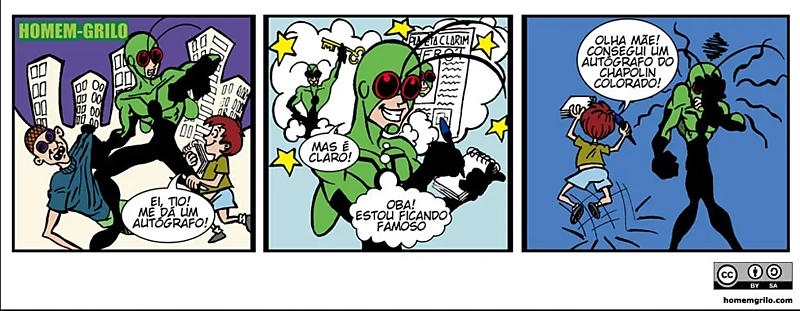
\includegraphics[width=5.40625in,height=1.77973in]{./imgSAEB_8_POR/media/image8.png}
\caption{Desenho de personagem de desenho animado}
% Descrição gerada
% automaticamente com confiança média
\end{figure}

\num{4} Em que consiste o humor presente na tirinha?

\reduline{O humor consiste no mal-entendido cometido pelo menino, que confundiu um
supér-herói com outro, deixando o homem-grilo aborrecido por não ter
sido reconhecido, como tinha pensado ser o caso.\hfill}
\linhas{4}

\num{5} Qual foi a expectativa criada pelo herói ao receber o pedido de
autógrafo e o que ele acaba descobrindo em relação a ela, no último
quadrinho?

\reduline{O personagem tinha a expectativa de que já era um super-herói famoso,
mas descobriu que ainda não tem fama.\hfill}
\linhas{4}

\num{6} A estratégia usada pelo autor da tirinha para gerar o humor é a
quebra de expectativa. Justifique essa afirmação.

\reduline{O personagem pensou ter sido reconhecido pelo menino como super-herói,
mas, após dar o autógrafo, teve sua expectativa quebrada, pois o menino
acaba revelando que o havia confundido com outro super-herói.\hfill}
\linhas{6}

\num{7} O que o mal-entendido cometido pelo menino revela sobre a
originalidade da fantasia do herói?

\reduline{O mal-entendido revela que o herói veste uma fantasia que o caracteriza
de forma pouco original.\hfill}
\linhas{4}

Leia as duas manchetes a seguir para resolver as atividades de 8 a 10.

\textbf{TEXTO I}

\begin{quote}
\textbf{Governo pretende lançar programa com passagens aéreas a R\$ 200}
\emph{Valor tem recorte de renda e categorias, como aposentados e
servidores}
\end{quote}

\fonte{Priscilla Mazenotti. Agência Brasil. Governo pretende lançar programa com passagens aéreas a R\$ 200. Disponível em: \url{https://agenciabrasil.ebc.com.br/radioagencia-nacional/economia/ervi/2023-03/programa-do-governo-preve-passagens-aereas-por-r-200}.
Acesso em: 14 mar. 2023.}

\textbf{TEXTO II}

\begin{quote}
\textbf{Governo quer lançar passagem aérea a R\$ 200 e ricos já cogitam
viajar de ônibus}
\end{quote}

\fonte{Sensacionalista. Governo quer lançar passagem aérea a R\$ 200 e ricos já cogitam viajar de ônibus. Disponível em: \url{https://oglobo.globo.com/blogs/humor/sensacionalista/post/2023/03/governo-quer-lancar-passagem-aerea-a-r-200-e-ricos-©-cogitam-viajar-de-onibus.ghtml}. Acesso em: 14 mar. 2023.}

\num{8} O texto II é uma versão humorística e fictícia da manchete de
notícia apresentada no texto I. Em que consiste o humor obtido no texto
II?

\reduline{O humor consiste no fato de a queda no valor da passagem aérea causar um
efeito contrário nos ricos, que passarão a viajar de ônibus, um
transporte popular por ser mais barato e, consequentemente, menos eficiente
no tempo de viagem.\hfill}
\linhas{6}

\num{9} O humor foi empregado no texto II com o objetivo de fazer uma
crítica social. Qual é essa crítica?

\reduline{A crítica social consiste no fato de os mais ricos não quererem se juntar aos mais pobres, que provavelmente viajarão mais de avião. Para evitar isso, preferirão viajar de ônibus, pois a queda no preço das passagens vai popularizar o transporte aéreo, sabidamente restrito à elite.\hfill}
\linhas{8}

\num{10} O que a fuga para o transporte rodoviário indica sobre a
satisfação dos ricos em relação à queda no preço da passagem aérea?
Justifique sua resposta.

\reduline{A fuga de um transporte de elite para um transporte popular indica que
os ricos têm uma opinião contrária e estão insatisfeitos com a queda dos
preços da passagem aérea, pois isso atrairá a população menos abastada
para esse tipo de transporte historicamente ocupado pela elite.\hfill}
\linhas{6}

\section{Treino}

\num{1} \textbf{Leia o texto.}

\begin{quote}
\textbf{Reunião de mães}
\end{quote}

\begin{quote}
Na reunião de pais só havia mães. Eu me sentiria constrangido em meio a
tanta mulher, por mais simpáticas que me parecessem, e acabaria nem
entrando --- se não pudesse logo distinguir, espalhadas no auditório,
duas ou três presenças masculinas {[}...{]}.
\end{quote}

\fonte{Fernando Pessoa. Reunião de mães. In: *O homem nu*. Rio de Janeiro: Record, 1976.}

O efeito de humor é obtido no texto a partir da presença de

\begin{escolha}
\item contradição.

\item ambiguidade.

\item situação absurda.

\item quebra de expectativa.
\end{escolha}

\num{2} Leia a manchete humorística.

\begin{quote}
\textbf{Autoridades aprendem com enxurradas e já começam a trabalhar em
desculpas para 2024}
\end{quote}

Sensacionalista. Autoridades aprendem com enxurradas e já começam a
trabalhar em desculpas para 2024. \fonte{Disponível em: \url{https://oglobo.globo.com/blogs/humor/sensacionalista/post/2023/02/autoridades-aprendem-com-enxurradas-e-comecam-a-trabalhar-em-desculpas-para-2024.ghtml}}.%linkquebrado
Acesso em: 06 mar. 2023.

O jornal \emph{Sensacionalista} se destaca pelo humor crítico em suas
notícias fictícias baseadas em notícias reais. O principal recurso usado
para provocar humor crítico nessa manchete é a

\begin{escolha}
\item ironia.

\item denúncia.

\item objetividade.

\item imparcialidade.
\end{escolha}

\num{3} \textbf{Leia o texto.}

\begin{quote}
\textbf{Conexão}
\end{quote}

\begin{quote}
Regido por esse despretensioso fluxo de ideias, me sinto tentado a fazer
uma parada. Até aqui me fiz tantas perguntas... Mas será que você,
leitor, é um jovem em busca de referências? Ou será que você é como eu
quando adolescente, que queria bater um papo sobre as identidades em
formação, mas sem um viés acadêmico? Só um papo que trouxesse conforto e
em que eu pudesse me espelhar... Quando, neste livro, eu sou você? Onde
nos encontramos? Em nossas semelhanças ou em nossas discordâncias?
\end{quote}

Lázaro Ramos. \emph{Na minha pele}. Rio de Janeiro: Objetiva, 2017.

Ao relatar sua busca por diálogos sobre as identidades em formação na
juventude, o autor emprega a expressão ``viés acadêmico'' para

\begin{escolha}
\item contrapor sua inquietude juvenil à sua passividade na vida adulta.

\item incentivar o leitor a dedicar-se ao estudo teórico do tema tratado.

\item caracterizar uma forma de abordagem com que ele não se identificava.

\item situar o tema no campo teórico em detrimento das experiências
vividas.
\end{escolha}

\chapter{Parcialidade em textos jornalísticos}
\markboth{Módulo 7}{}

\section{Habilidades do SAEB}

\begin{itemize}
\tightlist
\item
  Analisar marcas de parcialidade em textos jornalísticos.
\item
  Avaliar diferentes graus de parcialidade em textos jornalísticos.
\item
  Avaliar a fidedignidade de informações sobre um mesmo fato divulgado
  em diferentes veículos e mídias.
\end{itemize}

\conteudo{
Muitos textos jornalísticos fazem parte do grupo dos gêneros textuais
informativos e são centrados na informação a ser transmitida. Isso
pressupõe certo distanciamento do autor, isto é, menor presença de
marcas de subjetividade ou valoração, o que no jornalismo é chamado de
\textbf{imparcialidade}, porém, nesse campo da comunicação, há graus
variados de tratamento da informação, isto é, há diferentes níveis de
imparcialidade, conforme o foco dado pelo jornal aos diferentes aspectos
do fato abordado. Isso porque, além da função de informar, o jornalismo
tem também a função de formar opinião.

Sendo assim, nem sempre um texto jornalístico se limita a transmitir
informação. Há gêneros textuais jornalísticos que informam e opinam ao
mesmo tempo. Imparcialidade e \textbf{parcialidade}, portanto, são
características presentes no jornalismo, dependendo do gênero textual, e
referem-se à presença ou à ausência de valoração.

Notícia e reportagem, típicos do jornalismo, são dois exemplos de
gêneros em que ocorre variação no tratamento da informação e, assim, no
nível de imparcialidade. Na notícia, o jornalista privilegia a
informação e tenta manter um nível maior de imparcialidade. Na
reportagem, ele pode ser mais parcial, não só informando os fatos, mas
emitindo avaliação sobre eles, com a intenção de trazer sua visão
crítica da realidade, o que pode influenciar na formação da opinião do
leitor.

Parcialidade é um termo também conhecido como isenção e pode
manifestar-se de forma explícita, quando está visível nas marcas
linguísticas do texto, ou implícita, isto é, quando exige interpretação
por parte do leitor. Dessa forma, uma habilidade muito importante é a de
identificar a parcialidade em textos jornalísticos.}

\section{Atividades}

Leia o texto a seguir para resolver as atividades de 1 a 4.

\begin{quote}
\textbf{Quem oferecer menos leva a Amazônia}

O desmatamento na Amazônia está em constante crescimento, o que torna
cada vez mais improvável que o país cumpra a meta de redução
estabelecida para 2020. De acordo com os compromissos assumidos em 2010,
o Governo Federal estabeleceu a meta de limitar a perda anual da
cobertura florestal na Amazônia a 3.900 quilômetros quadrados até o
próximo ano. No entanto, em 2018, esse índice atingiu 7.900 quilômetros
quadrados, a maior taxa da década, e os sistemas de alerta indicam um
aumento de 20\% no desmatamento entre agosto de 2018 e abril de 2019.
Esses números evidenciam que o Brasil continua destruindo um de seus
recursos mais valiosos sem melhorar a qualidade de vida na região, que
continua apresentando indicadores socioeconômicos abaixo da média
nacional.

Esse processo de devastação ocorre devido à fragilização das políticas
públicas de controle do desmatamento, à falta de uma estratégia de
desenvolvimento para a região que valorize a preservação florestal e à
existência de leis federais e estaduais que incentivam a apropriação
ilegal de terras públicas, as quais são desmatadas para posterior
privatização. Na verdade, desde 2017, essas regras fundiárias que
estimulam o desmatamento vêm passando por preocupantes modificações,
muitas vezes despercebidas pela sociedade brasileira. Todas essas
alterações são justificadas em nome da modernização da regularização
fundiária e da redução da burocracia. No entanto, na prática, as novas
leis acabam favorecendo a grilagem de terras.

Além da modificação da lei federal, os estados da Amazônia também estão
promovendo uma série de alterações em suas regras fundiárias, seguindo a
mesma direção: legalizar o que era ilegal e incentivar o roubo de terras
públicas no futuro. A existência de leis em diferentes níveis de governo
ocorre porque a legislação federal se aplica apenas às terras
pertencentes à União, enquanto cada estado tem o poder de estabelecer
suas próprias regras para as áreas sob sua jurisdição. De acordo com
estimativas do Imazon, cerca de 33\% da Amazônia Legal não possui
destinação fundiária ou não há informações disponíveis publicamente
sobre o assunto. A maioria dessas áreas pertence aos estados (75\%).
Portanto, as regras estaduais têm um impacto ainda maior do que as
regras federais na determinação do destino de uma extensa área de
florestas públicas não designadas.
\end{quote}

\fonte{Fonte de pesquisa: Brenda Brito e Jeferson Almeida. El País. A Amazônia está à venda: quem der menos leva. Disponível em: \url{https://brasil.elpais.com/brasil/2019/06/19/opinion/1560981343_901218.html}. Acesso em: 17 maio 2023.}

\num{1} Qual é o fato que está sendo abordado no texto?

\reduline{O fato abordado são as mudanças que estão sendo feitas nas leis federais
e estaduais que versam sobre florestas públicas e a Amazônia. O texto é
claramente opinativo, porém ele se baseia em um fato objetivo (as leis
federais e estaduais que vêm sofrendo mudanças), sobre o qual os autores passam
a opinar e fazer avaliações.\hfill}
\linhas{8}

\num{2} O fato é abordado com parcialidade ou imparcialidade? Justifique
sua resposta com um exemplo extraído do texto.

\reduline{O fato (as leis federais e estaduais que vêm sofrendo mudanças) é claramente
abordado com imparcialidade, pois os autores passam a avaliar essas mudanças
como prejudiciais à proteção das florestas públicas, sobretudo da
Amazônia. Os elementos do texto que comprovam a imparcialidade são, por exemplo:
"estimulam o roubo de florestas públicas", "quem oferecer menos leva a Amazônia".\hfill}
\linhas{10}

\num{3} Conforme sua resposta à questão anterior, esse texto
jornalístico aproxima-se melhor de uma notícia ou de uma reportagem?
Justifique sua resposta.

\reduline{O texto aproxima-se melhor de uma reportagem, pois o trecho apresentado
tem uma estrutura semelhante à de uma notícia, diferenciando-se dela por abordar um fato relevante para a sociedade e emitindo parecer sobre ele, cumprindo a função jornalística de formar opinião.\hfill}
\linhas{10}

\num{4} O título do texto apresenta uma ironia que se constrói por meio
de uma contradição. Explique essa contradição.

\reduline{A contradição está no fato de se colocar à venda algo tão valioso como a
Amazônia e aceitar o menor valor pela venda dela.\hfill}
\linhas{4}

Leia as manchetes a seguir para resolver as atividades de 5 a 10. As
manchetes foram adaptadas de jornais que circulam no estado de Minas
Gerais.

\textbf{TEXTO I}

\begin{quote}
\textbf{Homem tenta serrar fio de alumínio e morre eletrocutado no
Betânia, em Belo Horizonte}
\end{quote}

\textbf{TEXTO II}

\begin{quote}
\textbf{Homem tenta furtar fios de cobre e morre eletrocutado em Belo
Horizonte}
\end{quote}

\textbf{TEXTO III}

\begin{quote}
\textbf{Homem morre eletrocutado em cima de poste em Belo Horizonte: a
suspeita é que ele tentava roubar a fiação}
\end{quote}

\num{5} Considerando as três manchetes como um todo, que fato está sendo
noticiado?

\reduline{O fato que certamente aconteceu é a morte de um homem eletrocutado.\hfill}
\linhas{2}

\num{6} Quais são os termos e expressões que sinalizam que os veículos
de imprensa apresentaram versões diferentes do mesmo fato? Compare os
textos I e II.

\reduline{O texto I diz que o homem tentou serrar os cabos e que esses cabos eram
de alumínio, enquanto o texto II acrescenta que ele tentou furtá-los e que
eles eram de cobre.\hfill}
\linhas{6}

\num{7} Entre os textos I e II, em qual está dito um provável motivo
para o homem se arriscar a ter contato com um fio eletrizado? Justifique
sua resposta.

\reduline{O texto II traz um provável motivo para o homem se arriscar a
ter contato com um fio eletrizado, pois diz que ele tentou furtar os
fios; portanto o furto foi o motivo que o levou a se arriscar.\hfill}
\linhas{4}

\num{8} Em relação ao tratamento do fato e à motivação do homem, qual é
a diferença do texto III para os textos I e II?

\reduline{O texto III trata a morte como fato e o furto como hipótese, enquanto os textos I e II não fazem essa distinção.\hfill}
\linhas{4}

\num{9} Qual das três manchetes atende melhor aos parâmetros do
jornalismo? Justifique sua resposta.

\reduline{O texto III é o que melhor atende aos parâmetros do jornalismo, pois
apresenta o fato com objetividade e imparcialidade, evitando afirmar
categoricamente que o homem tentava roubar os fios e buscando manter no campo da hipótese para que não soe como acusação leviana.\hfill}
\linhas{8}

\num{10} Por todas as características abordadas nas atividades
anteriores, na sua opinião, qual das três manchetes apresenta maior
imparcialidade? Justifique sua resposta.

\reduline{Resposta pessoal. Uma hipótese plausível de resposta, com base na
abordagem feita às caraterísticas dos textos, é apontar o texto III.\hfill}
\linhas{4}

\section{Treino}

\num{1} \textbf{Leia o texto.}

\begin{quote}
\textbf{Ipea: população em situação de rua no Brasil supera 281 mil}
\end{quote}

\begin{quote}
\emph{Em dez anos, esse segmento vulnerável cresceu 211\%}
\end{quote}

\begin{quote}
{[}\ldots{]}

O estudo do Ipea alerta que o aumento de pessoas nas ruas é muito maior
em proporção do que o da população em geral. No período de dez anos, de
2012 a 2022, o crescimento desse segmento vulnerável foi de 211\%.
Segundo dados do IBGE, o aumento populacional brasileiro foi de 11\%
entre 2011 e 2021.

A Região Sudeste concentra pouco mais da metade da população em situação
de rua do país: são 151 mil pessoas. Na sequência estão Nordeste, Sul,
Centro-Oeste e Norte. A pesquisa destaca a Região Norte, onde está a
menor parcela de população de rua do país {[}...{]}.
\end{quote}

\fonte{Gabriel Brum. Agência Brasil. Ipea: população em situação de rua no Brasil supera 281 mil. Disponível em: \url{https://agenciabrasil.ebc.com.br/direitos-humanos/noticia/2023-02/ipea-populacao-em-situacao-de-rua-no-brasil-supera-281-mil}. Acesso em: 05 mar. 2023.}

A expressão ``população em situação de rua'' é uma escolha alternativa
para referir-se aos indivíduos antes referidos como ``moradores de rua''
ou ``mendigos''. O uso dessa expressão no texto está pautado na ideia de

\begin{escolha}

\item linguagem neutra, que trata a todos de maneira igualitária.

\item compaixão, para ressaltar a vulnerabilidade dessas pessoas.

\item condição temporária, isto é, ``estar na rua'' e não ``ser da rua''.

\item solidariedade, para aumentar a adesão às campanhas de doação.

\end{escolha}

\num{2} Leia as manchetes a seguir.

\textbf{TEXTO I}

\begin{quote}
\textbf{Greve do Metrô é mantida para a semana do Carnaval}
\emph{Metroviários de Belo Horizonte decidiram manter a greve do Metrô
após assembleia na noite desta terça-feira (14)}
\end{quote}

\fonte{Maria Cavalcanti. Itatiaia. Greve do Metrô é mantida para semana do Carnaval. Disponível em: \url{https://www.itatiaia.com.br/editorias/cidades/2023/02/14/greve-do-metro-e-mantida-para-semana-do-carnaval}. Acesso em: 05 mar. 2023.}

\textbf{TEXTO II}

\begin{quote}
\textbf{Serviço essencial deve ser prestado} \emph{Falta na greve do
Metrô, sobretuddo, a empatia: milhares de belo-horizontinos e turistas
estão privados, no Carnaval, de um meio de transporte fundamental}
\end{quote}

\fonte{O tempo. Serviço essencial deve ser prestado. Disponível em: \url{https://www.otempo.com.br/opiniao/editorial/servico-essencial-deve-ser-prestado-1.2817688}. Acesso em: 05 mar. 2023.}

Esses textos jornalísticos apresentam diferentes finalidades
comunicativas em razão de seus gêneros serem distintos. Os textos I e II
destinam-se, respectivamente, a

\begin{escolha}
\item divulgar a assembleia dos metroviários e criticar o evento.

\item informar sobre a manutenção da greve e avaliar essa decisão.

\item criticar os metroviários pela greve e reclamar da falta de
transporte.

\item avaliar a necessidade da greve e solidarizar-se com os prejudicados.
\end{escolha}

\num{3} Leia as manchetes a seguir.

\textbf{TEXTO I}

\begin{quote}
\textbf{Com Bolsonaro, desmatamento na Amazônia cresce 150\%, pior marca
já registrada pelo Imazon} \emph{Com devastação recorde em 2022,
floresta perdeu o equivalente aos estados de Alagoas e Sergipe nos
últimos quatro anos}
\end{quote}

 \fonte{Murilo Pajolla. Brasil de fato. Com Bolsonaro,
desmatamento na Amazônia cresce 150\%, pior marca já registrada pelo
Imazon. Disponível em:
\url{https://www.brasildefato.com.br/2023/01/20/com-bolsonaro-desmatamento-na-amazonia-cresce-150-pior-marca-©-registrada-pelo-imazon}.
Acesso em: 05 mar. 2023.}

\textbf{TEXTO II}

\begin{quote}
\textbf{A mídia mentiu: desmatamento na Amazônia cai mais de 11\% em
2022} \emph{O resultado positivo foi consequência do trabalho de
diferentes órgãos do Governo Federal na Operação Guardiões}
\end{quote}

 \fonte{Redacción Brasil. Jornal Direita. A mídia mentiu:
desmatamento na Amazônia cai mais de 11\% em 2022. Disponível em:
\emph{\url{https://jornaldireita.com.br/a-midia-mentiu-desmatamento-na-amazonia-cai-mais-de-11-em-2022/}}.
Acesso em: 05 mar. 2023.}

As manchetes apresentadas nos textos I e II versam sobre o mesmo fato.
Ao compará-las, o leitor em busca de se informar sobre o assunto terá de
lidar com a dúvida sobre

\begin{escolha}
\item o momento em que ocorreu o fato noticiado.

\item a ocorrência do fato noticiado: o desmatamento.

\item as taxas reais de aumento e queda do desmatamento.

\item os posicionamentos políticos assumidos pelos veículos.
\end{escolha}

\chapter{Modalização}
\markboth{Módulo 8}{}

\section{Habilidades do SAEB} 

\begin{itemize}
  \item Identificar os recursos de modalização
em textos diversos. 
\item Analisar os efeitos de sentido dos tempos, modos
e/ou vozes verbais com base no gênero textual e na intenção
comunicativa. - Analisar os efeitos de sentido produzidos pelo uso de
modalizadores em textos diversos.
\end{itemize}

\subsection{Habilidades da BNCC}

\begin{itemize}
\tightlist
\item
  EF69LP04, EF69LP28, EF89LP16, EF89LP31, EF08LP16.
\end{itemize}

\conteudo{Um texto é muito mais que um simples conjunto organizado de palavras e
enunciados combinados. Por trás desse conjunto que chamamos de texto
está a escolha feita entre infinitas possibilidades de combinação e
seleção de palavras e frases. É justamente nas possibilidades de escolha
e combinação que o autor pode interferir, para moldar seu texto segundo
diferentes objetivos.

Essa intervenção deixa marcas que permitem perceber as atitudes do autor
em relação àquilo que está dizendo e o direcionamento argumentativo que
pretende dar ao texto. Chamamos essas marcas de \textbf{modalizadores do
discurso}. Em resumo, modalizadores são as marcas linguísticas que
revelam a atitude do autor em relação ao que ele diz, revelando,
portanto, a subjetividade de quem fala ou escreve. Essas atitudes podem
ser, por exemplo, de crítica, elogio, análise/julgamento, delimitação,
sentimento, intenção, desejo, vontade, necessidade, obrigatoriedade,
certeza, dúvida, possibilidade, proibição, permissão, crença.}

\section{Atividades}

\num{1} Explicite o sentido expresso pelas palavras modalizadoras em
destaque nas frases.

a) \textbf{Possivelmente}, aqui no Brasil, a melhor solução para os
alunos das redes públicas de ensino consistirá no uso de conteúdos
transmitidos por meio dos celulares com internet.

Trata-se de avaliação, possibilidade ou delimitação?

\reduline{Possibilidade.\hfill}
\linhas{1}

b) O secretário-geral das Nações Unidas, António Guterres, afirmou que
``\textbf{precisamos} alçar a voz contra todas as expressões de racismo
e casos de comportamento racista''.

Trata-se de avaliação, obrigação ou necessidade?

\reduline{Necessidade.\hfill}
\linhas{1}

c) A arte de viver cada vez mais se faz \textbf{indispensável} para a
emancipação humana.

Trata-se de necessidade, obrigação ou certeza?

\reduline{Necessidade.\hfill}
\linhas{1}

d) Hoje enfrentamos, em nosso país, árdua discussão sobre o uso do
ensino mediado por tecnologias. \textbf{Talvez} esse período nos ensine
que ambas as modalidades \textbf{podem} conviver em harmonia em prol de
um projeto pedagógico que atenda às necessidades de uma educação voltada
para o século XXI.

Trata-se de julgamento, obrigação ou hipótese?

\reduline{Hipótese.\hfill}
\linhas{1}

e) \textbf{Estranhamente}, a cada temporada, os eleitores teimam em
repetir erros grosseiros, votando em candidatos que, lá na frente,
voltam a atentar contra a cidadania.

Trata-se de delimitação, julgamento ou certeza?

\reduline{Julgamento.\hfill}
\linhas{1}

\num{2} Numerando-os, classifique os itens pelo posicionamento do
falante em relação ao que diz.

\begin{multicols}{2}

I. Obrigatoriedade. 
II. Proibição. 
III. Permissão.

\columnbreak

( \rosa{II} ) É vedado ao assistente social praticar condutas
antiéticas. 
( \rosa{III} ) Você pode sair hoje à noite com seus
amigos. 
( \rosa{I} ) Você deve fazer as tarefas de casa.
\end{multicols}

\num{3} Adicione modalizadores às frases de acordo com o sentido
indicado entre parênteses.

a) Ele acredita demais nas próprias verdades. (Hipótese)

\reduline{Possibilidade de resposta: Talvez ele acredite demais nas próprias verdades.\hfill}
\linhas{3}

b) Ele viu o gabarito antes da prova. (Incerteza)

\reduline{Possibilidade de resposta: Parece que ele viu o gabarito antes da prova.\hfill}
\linhas{3}

c) Eu vou chegar à escola às 7h. (Necessidade)

\reduline{Possibilidade de resposta: Eu preciso chegar à escola às 7h.\hfill}
\linhas{3}

d) Não tirou boa nota na escola este ano. (Julgamento)

\reduline{Possibilidade de resposta: Infelizmente, não tirou boa nota na escola este ano.\hfill}
\linhas{3}

e) João viajará de avião por temer o perigo das estradas.
(Probabilidade)

\reduline{Possibilidade de resposta: João provavelmente viajará de avião por temer o perigo das estradas.\hfill}
\linhas{3}

\num{4} Aponte, em cada texto, a palavra ou expressão que permite
identificar a atitude de quem fala frente ao que é dito. Em seguida,
justifique a resposta.

a) Um banho quente de chuveiro elétrico de 15 minutos consome 135 litros
de água. Um banho de 5 minutos, com o registro fechado para ensaboar,
consome apenas 45 litros.

\reduline{A palavra é "apenas". O locutor avalia uma atitude em relação a outra no
uso de água, realçando uma delas como a mais adequada para a economia de
água.}
\linhas{4}

b) Ainda é cedo para afirmar quais são os verdadeiros impactos da
sociedade tecnológica.

\reduline{A expressão é ``ainda é cedo''. O locutor alerta
que pode ser leviano fazer uma afirmação sobre os impactos da sociedade
tecnológica.\hfill}
\linhas{4}

c) O controle de dados dos internautas pode ser utilizado como artifício
para manipular a opinião desse público.

\reduline{A expressão é "pode ser". O locutor evita generalizar que todo controle
de dados é usado para fins negativos de manipulação, expressando assim
que o uso para essa finalidade é uma das possibilidades, que podem
também ser positivas.\hfill}
\linhas{4}

d) Sim! Foi a Tara Sports, usando a imagem de Ronaldo Fenômeno, que
salvou o Cruzeiro de um buraco ainda maior em 2022.

\reduline{A palavra é "sim". Trata-se de uma afirmação categórica que se
antecipa ao teor do que está sendo confirmado pela palavra, demonstrando
que o locutor acredita piamente no que diz e pretende que seu leitor
também acredite.\hfill}
\linhas{4}

\num{5} Escreva sentenças que expressem as atitudes indicadas a seguir.

a) Certeza.

\reduline{Resposta pessoal.\hfill}
\linhas{3}

b) Incerteza.

\reduline{Resposta pessoal.\hfill}
\linhas{3}

c) Hipótese.

\reduline{Resposta pessoal.\hfill}
\linhas{3}

d) Necessidade.

\reduline{Resposta pessoal.\hfill}
\linhas{3}

e) Obrigação.

\reduline{Resposta pessoal.\hfill}
\linhas{3}

f) Análise/julgamento.

\reduline{Resposta pessoal.\hfill}
\linhas{3}

Leia o texto a seguir para resolver as atividades de 6 a 8.

\begin{quote}
A informação está cada vez mais ao nosso alcance. Mas a sabedoria, que é
o tipo mais precioso de conhecimento, essa só pode ser encontrada nos
grandes autores da literatura.
\end{quote}

\fonte{W. R. Cereja e T. C. Magalhães. *Português:* linguagens. São Paulo:
Atual, 2012.}

\num{6} Qual é o assunto principal do texto?

\reduline{O assunto do texto é o valor da informação comparado ao valor da
sabedoria.\hfill}
\linhas{2}

\num{7} A parcialidade é uma característica presente no texto. Qual é a
opinião que o texto traz sobre o assunto tratado?

\reduline{A opinião expressa é a de que a sabedoria vale mais que a informação,
pois esta é trivial, por sua presença maciça e pela facilidade de alcance por
todos, enquanto aquela está restrita à literatura de grandes autores, demandando maior esforço para ser adquirida.\hfill}
\linhas{6}

\num{8} Qual é o efeito de sentido provocado pelos elementos
linguísticos ``mas'' e ``só'' na construção da opinião presente no
texto? Explique.

\reduline{O articulador "mas" expressa sentido oposto ao que foi dito na frase
anterior, e com ele o texto atribui valor especial à sabedoria em
oposição à trivialidade da informação. O termo "só" reforça que a
sabedoria é restrita a poucos, enquanto a informação é mais facilmente
acessível.\hfill}
\linhas{6}

\num{9} Para tentar combater o tabagismo, a Prefeitura de Araçás (um
município da Bahia) lançou um anúncio com estes dizeres:

\begin{quote}
Não deixe sua vida virar fumaça!
\end{quote}

O anúncio de que esse texto fazia parte celebrava o dia 31 de maio como
o dia mundial de combate ao fumo.

O texto utiliza-se da estratégia de abordar o leitor de forma menos
enfática e mais suave. Qual é a ordem ou recomendação enfática que foi
suavizada?

\reduline{A ordem é: Pare de fumar!\hfill}
\linhas{2}

\num{10} Ainda sobre o texto presente na atividade anterior, qual é o
efeito de sentido obtido no texto com a abordagem menos enfática do
leitor?

\reduline{O emprego de sentido conotativo, responsável pela abordagem menos
enfática ao leitor, gerou um efeito menos impositivo e autoritário no
texto, e assim pode contribuir para a adesão do leitor, por não ser
abordado de uma forma que pode lhe causar incômodo.\hfill}
\linhas{6}

\section{Treino}

Leia o texto e responda às questões de 1 a 3.

\begin{quote}
\textbf{Manaus sofre com expansão urbana em assentamentos precários}
\emph{Crescimento desordenado favorece ocorrência de desastres naturais}
\end{quote}

\begin{quote}
Um estudo publicado recentemente pela rede colaborativa de organizações
não governamentais (ONGs) MapBiomas mostra que Manaus é a cidade com
maior expansão das áreas urbanizadas em assentamentos precários no país.
A ocupação desordenada em áreas de risco trouxe problemas ambientais
graves, como a ocorrência de desastres naturais e outros processos de
degradação ambiental causados pela ação do homem. {[}\ldots{]} um
deslizamento de terra na capital amazonense atingiu 11 casas do bairro
Jorge Teixeira, na zona leste da cidade, e deixou oito mortos. O
prefeito David Almeida decretou estado de calamidade pública.
\end{quote}

\begin{quote}
Em razão dessa tragédia, a MapBiomas reuniu dados específicos do bairro
onde ocorreram as fatalidades para verificar a evolução de áreas
urbanizadas em Manaus. ``Especificamente na Rua Pingo D'agua, no Bairro
Jorge Teixeira em Manaus, onde ocorreu a morte de oito pessoas devido a
um deslizamento de terra, não havia registro de área de risco
cadastrada. No entanto, a área encontra-se dentro de um assentamento
precário conhecido e delimitado pelo IBGE'', aponta o estudo.
\end{quote}

\begin{quote}
{[}\ldots{]}
\end{quote}

\fonte{Pedro Lacerda. Agência Brasil. Manaus sofre com expansão urbana em assentamentos precários. Disponível em: \url{https://agenciabrasil.ebc.com.br/geral/noticia/2023-03/manaus-sofre-com-expansao-urbana-em-assentamentos-precarios}. Acesso em: 19 mar. 2023.}

\num{1} O texto privilegia na manchete o emprego de verbos no tempo
presente, produzindo o efeito de

\begin{escolha}
\item atualidade dos fatos noticiados.

\item comprovação da veracidade dos fatos.

\item imparcialidade na abordagem dos fatos.

\item apreciação sobre os fatos noticiados.
\end{escolha}

\num{2} Os termos ``expansão urbana'' e ``crescimento desordenado'', ao
revelarem posicionamentos distintos em relação ao mesmo fato,
exemplificam o fenômeno da

\begin{escolha}
\item veracidade.

\item modalização.

\item objetividade.

\item imparcialidade.
\end{escolha}

\num{3} A transmissão de informações sobre o fato mescla-se, no texto,
com a emissão de posicionamento do veículo, manifestado

\begin{escolha}
\item na linguagem desinteressada com que o fato é abordado.

\item no emprego da primeira pessoa para marcar a pessoalidade.

\item na citação de um estudo desenvolvido pela ONG MapBiomas.

\item na visão pessimista sobre o crescimento da cidade de Manaus.
\end{escolha}

\chapter{Figuras de linguagem}
\markboth{Módulo 9}{}

\section{Habilidades do SAEB}

\begin{itemize}
\tightlist
\item
  Analisar o uso de figuras de linguagem como estratégia argumentativa.
\item
  Avaliar a eficácia das estratégias argumentativas em textos de
  diferentes gêneros.
\end{itemize}

\subsection{Habilidades da BNCC}

\begin{itemize}
\tightlist
\item
  EF69LP17, EF89LP06, EF89LP14, EF89LP37.
\end{itemize}

\conteudo{
As figuras de linguagem podem ser recursos muito úteis nos textos
argumentativos. Elas se caracterizam por expressarem sempre um sentido
figurado, mas não se restringem aos textos literários. Por darem
dinâmica e maior força à construção de sentidos em um texto,
consequentemente podem auxiliar o autor na tarefa de argumentar,
persuadir, convencer.

Figuras de linguagem são recursos que permitem tornar o texto mais rico
e interessante, pois provocam um deslocamento do sentido literal para o
sentido figurado, isto é, trata-se de uma fuga da expressão comum para
uma expressão inovadora, o que enriquece a linguagem.

São várias as figuras de linguagem, mas aqui vamos nos ater às mais
importantes, cujo caráter argumentativo é mais perceptível e recorrente
em textos argumentativos.}

\begin{longtable}[]{@{}lll@{}}
\toprule
\begin{minipage}[b]{0.29\columnwidth}\raggedright
\textbf{Figura de linguagem}\strut
\end{minipage} & \begin{minipage}[b]{0.29\columnwidth}\raggedright
\textbf{Conceito}\strut
\end{minipage} & \begin{minipage}[b]{0.29\columnwidth}\raggedright
\textbf{Exemplo}\strut
\end{minipage}\tabularnewline
\midrule
\endhead
\begin{minipage}[t]{0.29\columnwidth}\raggedright
Comparação\strut
\end{minipage} & \begin{minipage}[t]{0.29\columnwidth}\raggedright
É a relação de semelhança entre elementos, por meio de um item
linguístico que promova uma comparação explícita.\strut
\end{minipage} & \begin{minipage}[t]{0.29\columnwidth}\raggedright
1) O teu olhar é fulminante \textbf{como} um raio.

2) Ele fala \textbf{que nem} papagaio.\strut
\end{minipage}\tabularnewline
\begin{minipage}[t]{0.29\columnwidth}\raggedright
Metáfora\strut
\end{minipage} & \begin{minipage}[t]{0.29\columnwidth}\raggedright
É o desvio da significação própria de uma palavra por meio de uma
comparação mental ou característica comum entre dois seres ou
fatos.\strut
\end{minipage} & \begin{minipage}[t]{0.29\columnwidth}\raggedright
Toda profissão tem seus espinhos.\strut
\end{minipage}\tabularnewline
\begin{minipage}[t]{0.29\columnwidth}\raggedright
Ironia\strut
\end{minipage} & \begin{minipage}[t]{0.29\columnwidth}\raggedright
É sugerir o contrário do que as palavras ou frases exprimem, quase
sempre com intenção sarcástica.\strut
\end{minipage} & \begin{minipage}[t]{0.29\columnwidth}\raggedright
Vejam os grandes feitos destes senhores: arruinar os bens públicos e
estimular a corrupção.\strut
\end{minipage}\tabularnewline
\begin{minipage}[t]{0.29\columnwidth}\raggedright
Metonímia\strut
\end{minipage} & \begin{minipage}[t]{0.29\columnwidth}\raggedright
Consiste em usar uma palavra no lugar de outra por causa da afinidade de
sentido entre elas, o que não significa que sejam sinônimas.\strut
\end{minipage} & \begin{minipage}[t]{0.29\columnwidth}\raggedright
Ele não tinha teto onde se abrigasse.\strut
\end{minipage}\tabularnewline
\begin{minipage}[t]{0.29\columnwidth}\raggedright
Eufemismo\strut
\end{minipage} & \begin{minipage}[t]{0.29\columnwidth}\raggedright
Consiste em suavizar a expressão de uma ideia triste ou desagradável,
substituindo por um termo polido menos impactante.\strut
\end{minipage} & \begin{minipage}[t]{0.29\columnwidth}\raggedright
O político faltou com a verdade.\strut
\end{minipage}\tabularnewline
\begin{minipage}[t]{0.29\columnwidth}\raggedright
Hipérbole\strut
\end{minipage} & \begin{minipage}[t]{0.29\columnwidth}\raggedright
Consiste no exagero da expressão.\strut
\end{minipage} & \begin{minipage}[t]{0.29\columnwidth}\raggedright
Já foi falado mais de mil vezes.\strut
\end{minipage}\tabularnewline
\begin{minipage}[t]{0.29\columnwidth}\raggedright
Antítese\strut
\end{minipage} & \begin{minipage}[t]{0.29\columnwidth}\raggedright
Consiste na colocação de duas ideias opostas lado a lado, no mesmo
enunciado.\strut
\end{minipage} & \begin{minipage}[t]{0.29\columnwidth}\raggedright
Não sei se gosto mais do dia, não sei se gosto mais da noite.\strut
\end{minipage}\tabularnewline
\begin{minipage}[t]{0.29\columnwidth}\raggedright
Gradação\strut
\end{minipage} & \begin{minipage}[t]{0.29\columnwidth}\raggedright
Consiste numa sequência de ideias colocadas em ordem crescente ou
decrescente de intensidade.\strut
\end{minipage} & \begin{minipage}[t]{0.29\columnwidth}\raggedright
Você tira o lixo de casa, da rua, do bairro, da cidade e até do país,
mas não tira do planeta.\strut
\end{minipage}\tabularnewline
\begin{minipage}[t]{0.29\columnwidth}\raggedright
Prosopopeia\strut
\end{minipage} & \begin{minipage}[t]{0.29\columnwidth}\raggedright
Consiste na atribuição de características humanas a seres
inanimados.\strut
\end{minipage} & \begin{minipage}[t]{0.29\columnwidth}\raggedright
``E o canto daquela guitarra estrangeira era um lamento choroso e
dolorido.'' (Aluísio Azevedo)\strut
\end{minipage}\tabularnewline
\begin{minipage}[t]{0.29\columnwidth}\raggedright
Catacrese\strut
\end{minipage} & \begin{minipage}[t]{0.29\columnwidth}\raggedright
Consiste em dar um novo sentido a uma palavra já existente, fazendo com
que ela passe a dar nome a outro ser, como se fosse um empréstimo
linguístico.\strut
\end{minipage} & \begin{minipage}[t]{0.29\columnwidth}\raggedright
Ele colocou um dente de alho no arroz.\strut
\end{minipage}\tabularnewline
\bottomrule
\end{longtable}

\section{Atividades}

Nas próximas atividades, omeie a figura de linguagem presente em cada
texto e justifique a presença dela, mostrando como se dá o teor
argumentativo em cada caso.

\num{1} Parabéns à Argentina, que bateu o recorde com a maior inflação
em 31 anos. Convenhamos: 102\% de inflação em 12 meses não é para
qualquer um.

\reduline{Ironia. A inflação, algo que é prejudicial à economia de um país, é
tratada como se fosse algo bom, equiparado a um recorde, mas a intenção
do autor é dizer justamente o contrário.\hfill}
\linhas{4}

\num{2} O meio ambiente pede socorro!

\reduline{Prosopopeia. O meio ambiente ganha expressão humana ao pedir
socorro, como forma de reforçar o perigo que a natureza está correndo.\hfill}
\linhas{4}

\num{3} Vida ou morte são situações corriqueiras na vida de médicos e
veterinários.

\reduline{Antítese. A figura de linguagem está representada na presença dos
termos opostos "vida" e "morte", o que pretende, por exemplo, reforçar a importância e, ao mesmo tempo, a dificuldade das profissões mencionadas.\hfill}
\linhas{4}

\num{4} Fui tão feliz naquela época. Eu vivia no paraíso e não sabia!

\reduline{Metáfora. O momento feliz é comparado a uma vida no paraíso, símbolo
de uma vida livre de problemas e cheia de felicidade, e isso dá muita expressividade ao momento de felicidade.\hfill}
\linhas{4}

\num{5} ``coube-me a boa fortuna de não comprar o pão com o suor do meu
rosto.'' (Machado de Assis)

\reduline{Metonímia. O pão representa o alimento do dia a dia e o suor
representa o trabalho. Com esses usos, o texto ganha força argumentativa ao mostrar que os dois elementos se opõem.\hfill}
\linhas{4}

\num{6} Eu já te falei um milhão de vezes que eu não gosto disso!

\reduline{Hipérbole. O exagero ocorre ao quantificar um número de vezes
impossível de alguém dizer algo. Nesse caso, o exagero gera uma argumentação mais forte.\hfill}
\linhas{4}

\num{7} Ela murmurou, sussurrou, falou, gritou, berrou\ldots{} já não
havia mais nada que pudesse fazer.

\reduline{Gradação. Os termos "gritar", "falar" e "murmurar" são variações de
uma mesma forma de expressão oral, significando que a personagem tentou
todas as possibilidades frente a alguma situação não citada na frase. A gradação é responsável por mostrar que as possibilidades de ação se esgotaram.\hfill}
\linhas{4}

\num{8} Os pais normalmente odeiam que as crianças se sentem no braço do
sofá.

\reduline{Catacrese. A parte do sofá chamada "braço" exemplifica o emprego
dessa palavra fora de seu uso original.\hfill}
\linhas{4}

\num{9} Aquela casa parece um campo de batalha!

\reduline{Comparação. A comparação entre a casa e o hospício significa que as
pessoas que ali moram se comportam de modo hostil. A construção da imagem reforça a ideia.\hfill}
\linhas{4}

\num{10} O réu faltou com a verdade no julgamento.

\reduline{Eufemismo. O eufemismo "faltar com a verdade" é uma forma de evitar
usar uma expressão mais pesada, como "mentir".\hfill}
\linhas{4}

\section{Treino}

\num{1} \textbf{Leia o texto.}

\begin{quote}
\textbf{O exercício da incerteza}
\end{quote}

\begin{quote}
Enquanto minha mãe era velada na sala de casa, tia Leonor me trocou a
roupa e disse: ``A mamãe descansou''. Fiquei sem saber o que pensar;
tinha apenas quatro anos, mas imaginei que descansar devia ser uma coisa
ruim, porque todos choravam.
\end{quote}

\begin{quote}
Passadas algumas semanas, senti uma tristeza doída no café da manhã
enquanto vó Aurélia fervia o leite, de costas para mim. ``Vó, nunca mais
vou ver a minha mãe?''
\end{quote}

\begin{quote}
Ela ouviu em silêncio, sem se virar para mim. Tinha lágrimas nos olhos
quando consegui ver seu rosto.
\end{quote}

\fonte{Drauzio Varella. *O exercício da incerteza:* Memórias. São Paulo: Companhia das Letras, 2022.}

No contexto apresentado, o uso da expressão ``A mamãe descansou'' teve o
objetivo de

\begin{escolha}
\item esconder do menino a notícia da morte da mãe.

\item confortar o menino em relação à morte da mãe.

\item provocar no menino o sentimento de perda da mãe.

\item explicar ao menino o sentido real do descanso da mãe.
\end{escolha}

\num{2} Leia o poema.

\begin{quote}
\textbf{XXI}

Se eu pudesse trincar a terra toda

E sentir-lhe um paladar,

Seria mais feliz um momento...

Mas eu nem sempre quero ser feliz.

É preciso ser de vez em quando infeliz

Para se poder ser natural...
\end{quote}

\begin{quote}
Nem tudo é dias de sol,

E a chuva, quando falta muito, pede-se.

Por isso tomo a infelicidade com a felicidade

Naturalmente, como quem não estranha

Que haja montanhas e planícies

E que haja rochedos e erva...
\end{quote}

\begin{quote}
{[}\ldots{]}
\end{quote}

\fonte{Fernando Pessoa. O guardador de rebanhos. In: *Poemas de Alberto Caeiro*. Disponível em: \url{http://arquivopessoa.net/textos/613}. Acesso em: 19 mar. 2023.}

A visão de mundo expressa no poema é construída linguisticamente a
partir de uma figura de linguagem caracterizada por

\begin{escolha}
\item emparelhar expressões opostas.

\item suavizar expressões impactantes.

\item exagerar o sentido das expressões.

\item inverter o sentido das expressões.
\end{escolha}

\num{3} \textbf{Leia o texto.}

\begin{quote}
\textbf{Obesidade infantil é tema do programa Salto para o Futuro}

Um dos problemas de saúde pública mais preocupantes atualmente, a
obesidade infantil, será o tema da próxima edição do
programa~\emph{Salto para o Futuro}, nesta quarta-feira, 18, às 20h, na
TV Escola. A escolha da matéria não acontece por acaso, uma vez que a
Organização Mundial de Saúde (OMS), em seu estudo mais recente, de
outubro de 2017, apontou um total de 124 milhões de crianças e
adolescentes obesos em todo o mundo.

{[}...{]}

As causas da doença e as medidas para evitar que crianças, adolescentes
e jovens se tornem obesos são o foco desta edição do programa da TV
Escola.
\end{quote}

\fonte{Ministério da Educação. Obesidade infantil é tema do programa Salto para o Futuro. Disponível em: \url{http://portal.mec.gov.br/ultimas-noticias/33491-tv-escola/63021-obesidade-infantil-e-tema-do-programa-salto-para-o-futuro}. Acesso em: 08 mar. 2023. (Adaptado.)}

Ao divulgar um programa de televisão, o texto menciona a Organização
Mundial de Saúde para

\begin{escolha}
\item informar a participação de um representante do órgão.

\item ressaltar a necessidade do combate à obesidade infantil.

\item influenciar a opinião do leitor sobre a obesidade infantil.

\item comprovar a pertinência e a importância do tema escolhido.
\end{escolha}

\chapter{Progressão textual}
\markboth{Módulo 10}{}

\section{Habilidade do SAEB}

\begin{itemize} 
\item Analisar os mecanismos que contribuem
para a progressão textual. 
\item Analisar os processos de referenciação
lexical e pronominal.
\end{itemize}

\subsection{Habilidades da BNCC}

\begin{itemize}
\tightlist
\item
  EF08LP13, EF08LP15.
\end{itemize}

\conteudo{A progressão textual é o desenvolvimento das ideias e do tema de um
texto. Esse desenvolvimento ocorre com a adição de informações novas às
informações já dadas, que precisam estar conectadas de modo que o texto
avance sem que o leitor perca a linha de raciocínio proposta pelo autor.

A coesão é a principal responsável pela adequada progressão temática,
pois estabelece relações entre diferentes partes e ideias do texto por
meio da \textbf{coesão referencial} e da \textbf{coesão sequencial},
retomando sem necessariamente repetir palavras e expressões do texto.}

\begin{itemize}
\item
  A coesão referencial ocorre quando um termo ou uma expressão refere-se
  a outro termo ou expressão dentro do texto, colaborando tanto para a
  manutenção quanto para a progressão do assunto. Alguns desses termos
  ou expressões são: pronomes, advérbios, numerais, artigos, sinônimos,
  antônimos, palavras genéricas, por exemplo.
\item
  A coesão sequencial ocorre com elementos linguísticos que estabelecem
  relações lógicas e semânticas entre as partes do texto. Esses
  elementos são chamados de conectivos e promovem a articulação entre
  ideias, informações e argumentos no texto.
\end{itemize}

\section{Atividades}

\num{1} Numere os enunciados de acordo com o valor semântico do termo
destacado.

\begin{multicols}{2}
I. Conclusão.

II. Contraste. 

III. Explicação.

IV. Confirmação. 

V. Síntese. 

VI. Destaque.

\columnbreak

(~\rosa{II} ) Conseguiu reaver o relógio, \textbf{contudo} o aparelho
estava quebrado. 

(~\rosa{VI} ) \textbf{Entre} os profissionais de
saúde que trabalharam na pandemia, vale ressaltar a coragem dos
enfermeiros que estiveram na linha de frente. 

(~\rosa{V} ) Um carro, uma casa, uma família linda, \textbf{tudo} parecia perfeito. 

(~\rosa{III} ) Queria comprar um vestido novo \textbf{porque} iria a uma
festa naquele dia. 

(~\rosa{IV} ) De fato o Brasil é o país do futebol

(~\rosa{I} ) Choveu bastante, portanto a colheita está garantida.
\end{multicols}

\num{2} Reescreva os enunciados ligando as orações por meio de
conectivos que expressem as ideias indicadas entre parênteses. Faça as
alterações necessárias.

a) Esforçou-se muito. Não teve sucesso. (Concessão)

\reduline{Possibilidade de resposta: Embora tenha se esforçado muito, não teve sucesso.\hfill}
\linhas{4}

b) Está chovendo. A roupa do varal ficou molhada. (Conclusão)

\reduline{Possibilidade de resposta: Está chovendo; portanto a roupa do varal ficou molhada.\hfill}
\linhas{4}

c) Gostamos de ler. Adoramos ouvir música. (Adição)

\reduline{Possibilidade de resposta: Gostamos de ler e adoramos ouvir música.\hfill}
\linhas{4}

d) Precisamos de um médico. Um cliente está passando mal. (Explicação)

\reduline{Possibilidade de resposta: Precisamos de um médico, pois um cliente está passando mal.\hfill}
\linhas{4}

\num{3} Complete a lacuna em cada frase com o conetivo adequado à ideia
indicada nos parênteses.

\_\_\_\_\_\_\_\_\_\_\_\_\_\_\_\_\_ \rosa{Embora} pertencêssemos a
partidos rivais, nossos ideais coincidiam em muitos pontos. (Concessão)

Ele disse que gostou muito do meu CD,
\_\_\_\_\_\_\_\_\_\_\_\_ \rosa{mas} com algumas ressalvas. (Contraste)

Irei contigo, \_\_\_\_\_\_\_\_\_\_\_\_\_\_\_\_ \rosa{caso} minha
família não se oponha. (Condição)

\textbf{Leia o texto a seguir para resolver as atividades de 4 a 9.}

\begin{quote}
No Brasil, há quase três décadas, os direitos civis, políticos e sociais
foram estabelecidos como garantidos. No entanto, para muitos cidadãos
brasileiros, essa garantia é mais evidente em teoria do que na prática.
Além disso, existe uma falta de alinhamento entre o que está previsto na
legislação e o que realmente acontece na sociedade brasileira.
\end{quote}

\fonte{Texto escrito para este material.}

%REVER, texto ficou menor a partir daqui
\num{4} O texto se abre com um fato e, na frase seguinte, é introduzida
uma problematização relativa a esse fato. Aponte essa problematização.

\reduline{A problematização é a falta da garantia dos direitos civis, políticos e
sociais para muitos brasileiros.\hfill}
\linhas{4}

\num{5} Indique o conectivo responsável por introduzir a problematização
apontada na atividade anterior e cite seu valor semântico.

\reduline{O conectivo é "no entanto".\hfill}
\linhas{1}

\num{6} Relacione o sentido expresso pelo conectivo à problematização
expressa na frase que ele introduz.

\reduline{O conectivo "no entanto" expressa oposição/contraste, e é exatamente
essa a ideia da frase que ele introduz, pois muitos
brasileiros, em quase trinta anos de garantia dos direitos civis, políticos e
sociais, ainda não têm esses direitos garantidos na prática, o que indica um
contraste entre a teoria e a realidade\hfill}
\linhas{6}

\num{7} \textbf{Releia um trecho.}

\begin{quote}
Além disso, existe uma falta de alinhamento entre o que está previsto na
legislação e o que realmente acontece na sociedade brasileira.
\end{quote}

Que valor o conectivo ``Além disso'' tem nesse contexto? Explique.

\reduline{O conectivo "Além disso" acrescenta uma ideia ao que vinha sendo desenvolvido no texto; tem, portanto, valor aditivo.\hfill}
\linhas{4}

\num{8} Indique os dois segmentos do texto que retomam, por meio de
paráfrase, as ideias dos termos ``teoria'' e ``prática''.

\reduline{As ideias das expressões "teoria" e "prática" são retomadas, respectivamente, pelos trechos "o que está previsto na legislação" "o que realmente acontece na sociedade brasileira".\hfill}
\linhas{4}

\num{9} O pronome demonstrativo ``isso'' promove uma economia
linguística no texto ao retomar, com apenas uma palavra, uma expressão
longa. Qual expressão o pronome está substituindo?

\reduline{O pronome "isso" retoma "essa garantia é mais evidente em teoria do que na prática".\hfill}
\linhas{4}

\num{10} \textbf{Leia o texto a seguir.}

\begin{quote}
\textbf{Desmatamento na Amazônia cai 36\% no primeiro quadrimestre}
\end{quote}

\begin{quote}
O tamanho da área desmatada na Amazônia durante os quatro primeiros
meses deste ano foi 36\% menor que no mesmo período de 2022, segundo
monitoramento do Instituto do Homem e Meio Ambiente da Amazônia
(Imazon), organização que desde 1990 reúne pesquisadores que se dedicam
a estudar aspectos relativos ao uso e conservação dos recursos naturais
da região.
\end{quote}

\begin{quote}
{[}\ldots{]}
\end{quote}

\begin{quote}
``A redução observada em abril é positiva, porém, a área desmatada no
mês ainda foi a quarta maior desde 2008 para o mês'', destaca a
pesquisadora Larissa Amorim, referindo-se aos resultados para o mesmo
mês registrados nos três anos anteriores: 1.197 km² (2022), 778 km²
(2021) e 529 km² (2020).
\end{quote}

\begin{quote}
``\textbf{Isso} indica que precisamos implantar ações emergenciais de
fiscalização, identificação e punição aos desmatadores ilegais nos
territórios mais pressionados, focando nas florestas públicas que ainda
não possuem uso definido e nas áreas protegidas, principalmente com a
chegada do verão amazônico, onde historicamente o desmatamento tende a
aumentar'', acrescenta Larissa, em nota divulgada pelo instituto.
\end{quote}

\begin{quote}
{[}\ldots{]}
\end{quote}

 \fonte{Alex Rodrigues. Agência Brasil. Desmatamento na
Amazônia cai 36\% no primeiro quadrimestre. Disponível em:
\url{https://agenciabrasil.ebc.com.br/geral/noticia/2023-05/desmatamento-na-amazonia-cai-36-no-primeiro-quadrimestre}.
Acesso em: 18 maio 2023.}

O que o pronome ``isso'' destacado no texto retoma?

\reduline{O pronome retoma a ideia de que, apesar de a redução observada em abril ser positiva, a área desmatada no mês ainda foi a quarta maior desde 2008.\hfill}
\linhas{4}

\section{Treino}

\num{1} \textbf{Leia o texto.}

\begin{quote}
{[}...{]}

Disse a mamãe, um dia, à loura Georgeana:

--- Se até anoitecer, eu não te ouvir chorar,

nem dar gritos, prometo, amor, ir-te comprar

uma nenê gentil, d'olhos de porcelana.

Apenas isto ouviu, a bela pequenita

dança e salta a cantar, com tal sofreguidão,

que entontecendo, cai, ao comprido, no chão.

Esqueceu-lhe a promessa. Ei-la que chora e grita.

--- Prantos? Adeus boneca. Ouvindo esta ameaça,

ergue-se Georgeana e diz muito ligeira,

mudando o choro em riso, e com imensa graça.

--- Chorei... por brincadeira...
\end{quote}

\fonte{Louis Ratisbonne. Tradução de Adelina Amélia Lopes Vieira. Disponível
em: \url{http://www.dominiopublico.gov.br/download/texto/wk000073.pdf}. Acesso
em: 11 fev.2023.}

No texto, a palavra que substitui o nome Georgeana e, ao mesmo tempo,
atribui uma característica à personagem é

\begin{escolha}
\item ``nenê''.

\item ``ligeira''.

\item ``boneca''.

\item ``pequenita''.
\end{escolha}

\num{2} \textbf{Leia o texto.}

\begin{quote}
\textbf{Uma soneca por todo o inverno}

Se alguém comentar: ``Você dorme como um urso!'', saiba que está
dormindo excessivamente. Afinal, os ursos têm a capacidade de dormir por
períodos extremamente longos. Na realidade, eles hibernam, ficando meses
sem acordar para comer, beber água ou se higienizar. Mas como os ursos e
outros animais conseguem fazer isso?

A natureza parece encontrar soluções para tudo. No inverno, os recursos
naturais diminuem. Basta observar as árvores, por exemplo, e perceber
que há menos folhas e menos frutas disponíveis. Nesse contexto, para
alguns animais, é mais vantajoso ``dormir'' durante esse período de
escassez alimentar.

É claro que dormir por um período tão prolongado requer algum tipo de
preparação. Nas estações que antecedem o inverno, os animais que
hibernam se preparam comendo em grande quantidade. Dessa forma, eles
acumulam reservas de energia na forma de gordura corporal. E, quando o
inverno chega, eles estão prontos para passar longos e frios meses em
suas tocas, até a chegada da primavera.
\end{quote}

\fonte{Fonte de pesquisa: Ciência Hoje das Crianças. Uma soneca por todo o inverno. Disponível em: \url{https://chc.org.br/artigo/uma-soneca-por-todo-o-inverno/}. Acesso em: 13 fev. 2023.}

A associação semântica entre os termos ``recursos naturais'', ``folhas''
e ``frutos'' permite identificar que, do primeiro para o segundo e o
terceiro, ocorre um movimento de

\begin{escolha}
\item oposição.

\item conclusão.

\item explicação.

\item particularização.
\end{escolha}

\num{3} \textbf{Leia o texto.}

\begin{quote}
As primeiras duas décadas do século XXI, no Brasil e no mundo
globalizado, foram marcadas por consideráveis avanços científicos,
dentre os quais destacam-se as tecnologias de informação e comunicação
(TICs). Nesse sentido, tal panorama promoveu a ampliação do acesso ao
conhecimento, por intermédio das redes sociais e mídias virtuais. Em
contrapartida, nota-se que essa realidade impôs novos desafios às
sociedades contemporâneas, como a possibilidade de manipulação
comportamental via dados digitais. Desse modo, torna-se premente
analisar os principais impactos dessa problemática: a perda da autonomia
de pensamento e a sabotagem dos processos políticos democráticos.
\end{quote}

\begin{quote}
{[}\ldots{]}
\end{quote}

\fonte{Pedro Assaad Salloum Moreira da Rocha. Disponível em:
\url{http://portal.mec.gov.br/images/stories/noticias/2019/outubro/24.10.2019redacaolink6.pdf}.
Acesso em: 21 fev. 2023.}

A problemática a que se refere o autor pode ser compreendida, no texto,
pela oposição entre

\begin{escolha}
\item Brasil e mundo globalizado.

\item redes sociais e mídias virtuais.

\item acesso ao conhecimento e manipulação comportamental.

\item perda da autonomia de pensamento e sabotagem dos processos políticos
democráticos.
\end{escolha}

\chapter{Variação linguística}
\markboth{Módulo 11}{}

\section{Habilidades do SAEB} 

\begin{itemize}
\item Analisar as variedades linguísticas em
textos.
\item Avaliar a adequação das variedades linguísticas em contextos
de uso.
\end{itemize}

\subsection{Habilidades da BNCC}

\begin{itemize}
\tightlist
\item
  EF69LP55, EF69LP56.
\end{itemize}

\conteudo{
A língua portuguesa é falada, no Brasil, por mais de 200 milhões de
pessoas, que podem ser agrupadas de acordo com as diferentes regiões do
país, os diferentes grupos sociais, as diferentes profissões, as
diferentes faixas de idade, os diferentes níveis de escolaridade, as
diferentes classes sociais, enfim, qualquer outro critério que possamos
determinar.

Mas será que, com tanta diversidade de grupos sociais, todas as pessoas
usam a língua da mesma forma? Será que você consegue identificar o grupo
a que uma pessoa pertence pelo modo como ela usa a língua? Claro que
sim! A língua pode variar de época para época, de região para região, de
classe social para classe social etc., e essas variações são um fenômeno
natural na língua. A variação, portanto, é parte integrante da língua.

Então será que existe um modo melhor ou mais correto de usar a língua?
Claro que não! A melhor variedade da língua será aquela mais adequada à
situação comunicativa. Portanto, todas as variedades de uso da língua
têm o mesmo valor, desde que sejam usadas na situação comunicativa
adequada.

As duas variedades de uso da língua mais comuns são a culta e a popular.
A variedade culta é usada por falantes escolarizados e está mais próxima
da norma-padrão ensinada nos livros de gramática usados na escola, pois
seu uso está baseado em regras gramaticais explícitas. A variedade
popular, por sua vez, é usada por falantes menos escolarizados e está
mais distante da norma-padrão ensinada nos livros, ignorando diversas
regras impostas nesses livros, por isso tende a sofrer preconceito
linguístico.

Essa situação é resultado de má interpretação e desconhecimento, pois as
pessoas pensam que a norma popular não tem regras e que somente a
norma-padrão é correta por seguir regras, o que é um conceito incorreto.
Toda manifestação da língua está pautada em regras internas do idioma,
regras naturais que organizam seus usos. A diferença entre a norma culta
e a norma popular é que a norma popular pauta o uso da língua em regras
não explícitas, enquanto a norma culta está preocupada em adequar-se a
regras conhecidas, isto é, explícitas. Caso não houvesse regras
gramaticais na norma popular, você não conseguiria compreender um
falante dessa variedade, e isso não é o que acontece na realidade.

Mas isso significa que pessoas escolarizadas só usem a variedade culta e
pessoas menos escolarizadas só usem a variedade popular, e que uma
variedade é melhor ou mais correta que a outra? Não! Todos nós usamos,
por exemplo, a variedade popular em algum momento, até mesmo com o
objetivo de nos adequarmos a uma situação comunicativa em que ela seja
necessária, provando assim que ela é uma variedade tão útil quanto a
variedade culta. Tanto as pessoas escolarizadas quanto as não
escolarizadas poderão usar ambas as variedades da língua conforme sintam
a necessidade de adequar sua linguagem ao contexto. A única diferença é
que as pessoas menos escolarizadas terão mais dificuldades em usar a
variedade culta, porque saber usá-la depende de ensino formal,
justamente por ser mais próxima da norma-padrão ensinada nos livros de
gramática.

Podemos, então, estabelecer uma importante diferença entre norma culta,
norma popular e norma-padrão: a norma culta é tipicamente falada por
pessoas escolarizadas; a norma popular é tipicamente falada por pessoas
não escolarizadas ou menos escolarizadas; e a norma-padrão é o conjunto
de regras de uso da língua ensinadas nos livros de gramática usados na
escola.

A variação linguística pode ser percebida por meio de marcas
linguísticas deixadas pelo falante. Vejamos agora alguns tipos de
variação linguística.}

\begin{longtable}[]{@{}ll@{}}
\toprule
\begin{minipage}[b]{0.46\columnwidth}\raggedright
\textbf{Variação linguística}\strut
\end{minipage} & \begin{minipage}[b]{0.46\columnwidth}\raggedright
Usos de uma língua que se diferenciam da norma-padrão influenciados por
convenções sociais, momento histórico, contexto ou região em que o
falante se encontra.\strut
\end{minipage}\tabularnewline
\midrule
\endhead
\begin{minipage}[t]{0.46\columnwidth}\raggedright
\textbf{Variação histórica}\strut
\end{minipage} & \begin{minipage}[t]{0.46\columnwidth}\raggedright
Influenciada pelo momento histórico da língua. Apresenta-se como
arcaísmo, isto é, uso de formas linguísticas que estão em desuso na
atualidade.

Exemplo: O português falado hoje no Brasil não é o mesmo falado no
Brasil Colônia.\strut
\end{minipage}\tabularnewline
\begin{minipage}[t]{0.46\columnwidth}\raggedright
\textbf{Variação geográfica (regional)}\strut
\end{minipage} & \begin{minipage}[t]{0.46\columnwidth}\raggedright
Influenciada pela localidade ou região de origem do falante.
Apresenta-se como sotaque e regionalismo.

Exemplo: O vocabulário regional gaúcho é diferente do vocabulário
regional mineiro, e vice-versa.\strut
\end{minipage}\tabularnewline
\begin{minipage}[t]{0.46\columnwidth}\raggedright
\textbf{Variação social}\strut
\end{minipage} & \begin{minipage}[t]{0.46\columnwidth}\raggedright
Influenciada pelo grupo social a que pertence o falante. Alguns exemplos
são profissão, classe social, nível de escolaridade, tribos urbanas,
idade, gênero. Apresenta-se como gíria e jargão.

Exemplo: As diferenças no modo de usar a língua entre pessoas de idades
diferentes, profissões diferentes, classes sociais diferentes etc.\strut
\end{minipage}\tabularnewline
\begin{minipage}[t]{0.46\columnwidth}\raggedright
\textbf{Variação situacional}\strut
\end{minipage} & \begin{minipage}[t]{0.46\columnwidth}\raggedright
Influenciada pela adequação da linguagem a determinada situação ou
contexto comunicativo. Exemplo: Os diferentes modos de falar que uma
mesma pessoa adota com os amigos e numa entrevista de emprego.\strut
\end{minipage}\tabularnewline
\bottomrule
\end{longtable}

O professor poderá explorar mais o assunto com debates em sala de aula,
baseando-se em filmes que mostrem variação linguística, música e outros
recursos que considerar convenientes, sempre trazendo à tona a questão
do preconceito linguístico e da valorização social diferente que é dada
às variedades da língua com base em critérios não linguísticos, mas
históricos, ideológicos, políticos e econômicos.

\section{Atividades}

\num{1} Conceitue norma-padrão, norma culta e norma popular.

%REVER, tem texto fora da tabela
\begin{longtable}[]{@{}lll@{}}
\toprule
Norma-padrão & Norma culta & Norma popular\tabularnewline
\midrule
\endhead
Conjunto de regras de uso da língua escritas no livro que se conhece
como gramática. & Modalidade da língua falada por pessoas residentes em
centros urbanos e com nível de escolaridade superior. & Modalidade da
língua falada pela população menos escolarizada, sobretudo no meio
rural.\tabularnewline
\bottomrule
\end{longtable}

\num{2} Conceitue variação linguística e cada tipo de variação
linguística: variação histórica, social, geográfica, social,
situacional.

\begin{longtable}[]{@{}ll@{}}
\toprule
Variação linguística &\tabularnewline
\midrule
\endhead
Variação histórica &\tabularnewline
Variação social &\tabularnewline
Variação geográfica &\tabularnewline
Variação situacional &\tabularnewline
\bottomrule
\end{longtable}

\begin{longtable}[]{@{}ll@{}}
\toprule
\begin{minipage}[b]{0.46\columnwidth}\raggedright
\textbf{Variação linguística}\strut
\end{minipage} & \begin{minipage}[b]{0.46\columnwidth}\raggedright
Usos de uma língua que se diferenciam da norma-padrão influenciados por
convenções sociais, momento histórico, contexto ou região em que o
falante se encontra.\strut
\end{minipage}\tabularnewline
\midrule
\endhead
\begin{minipage}[t]{0.46\columnwidth}\raggedright
\textbf{Variação histórica}\strut
\end{minipage} & \begin{minipage}[t]{0.46\columnwidth}\raggedright
Influenciada pelo momento histórico da língua. Apresenta-se como
arcaísmo, isto é, uso de formas linguísticas que estão em desuso na
atualidade.

Exemplo: O português falado hoje no Brasil não é o mesmo falado no
Brasil Colônia.\strut
\end{minipage}\tabularnewline
\begin{minipage}[t]{0.46\columnwidth}\raggedright
\textbf{Variação geográfica (regional)}\strut
\end{minipage} & \begin{minipage}[t]{0.46\columnwidth}\raggedright
Influenciada pela localidade ou região de origem do falante.
Apresenta-se como sotaque e regionalismo.

Exemplo: O vocabulário regional gaúcho é diferente do vocabulário
regional mineiro, e vice-versa.\strut
\end{minipage}\tabularnewline
\begin{minipage}[t]{0.46\columnwidth}\raggedright
\textbf{Variação social}\strut
\end{minipage} & \begin{minipage}[t]{0.46\columnwidth}\raggedright
Influenciada pelo grupo social a que pertence o falante. Alguns exemplos
são profissão, classe social, nível de escolaridade, tribos urbanas,
idade, gênero. Apresenta-se como gíria e jargão.

Exemplo: As diferenças no modo de usar a língua entre pessoas de idades
diferentes, profissões diferentes, classes sociais diferentes etc.\strut
\end{minipage}\tabularnewline
\begin{minipage}[t]{0.46\columnwidth}\raggedright
\textbf{Variação situacional}\strut
\end{minipage} & \begin{minipage}[t]{0.46\columnwidth}\raggedright
Influenciada pela adequação da linguagem a determinada situação ou
contexto comunicativo. Exemplo: Os diferentes modos de falar que uma
mesma pessoa adota com os amigos e numa entrevista de emprego.\strut
\end{minipage}\tabularnewline
\bottomrule
\end{longtable}

\num{3} Pense sobre os seguintes exemplos de preconceito linguístico e
responda.

\begin{itemize}
\item
  rir de alguém por causa do sotaque;
\item
  achar que o português falado em Portugal é mais correto que o falado
  \textgreater{} no Brasil;
\item
  debochar de quem usa gírias antigas;
\item
  corrigir a pronúncia ``errada'' de alguém;
\item
  acreditar que a linguagem usada antigamente era mais correta;
\item
  discriminar a linguagem simplificada usada na internet.
\end{itemize}

O preconceito linguístico realmente se justifica nessas situações, ou
esses usos devem ser entendidos como um fenômeno natural de variação da
língua? Justifique. (6 linhas)

\reduline{Esses usos devem ser entendidos como variação linguística, pois são
variedades que respeitam regras internas da língua portuguesa, assim
como outros usos mais valorizados socialmente, como, por exemplo, aquele
prescrito pela norma-padrão. Caso não respeitassem regra alguma, seriam
incompreensíveis a um falante da língua portuguesa.\hfill}
\linhas{6}

%REVER, tem texto fora da tabela
\num{4} Escreva o tipo de variação linguística representado em cada
situação de uso da língua e indique o fator que influencia a variação.

\begin{longtable}[]{@{}ll@{}}
\toprule
\textbf{Uso da língua} & \textbf{Tipo de variação
linguística}\tabularnewline
\midrule
\endhead
Falar com sotaque para marcar sua origem natal &\tabularnewline
Usar jargão médico para conversar com um colega enfermeiro
&\tabularnewline
Conversar com o avô e estranhar os termos que ele usa de determinada
época &\tabularnewline
Usar linguagem formal para participar de uma entrevista de emprego
&\tabularnewline
\bottomrule
\end{longtable}

\begin{longtable}[]{@{}ll@{}}
\toprule
\textbf{Uso da língua} & \textbf{Tipo de variação
linguística}\tabularnewline
\midrule
\endhead
Falar com sotaque para marcar sua origem natal & Variação geográfica
(influenciada pela região)\tabularnewline
Usar jargão médico para conversar com um colega enfermeiro & Variação
social (influenciada pela profissão)\tabularnewline
Conversar com o avô e estranhar os termos que ele usa de época passada &
Variação histórica (influenciada pelo momento histórico da
língua)\tabularnewline
Usar linguagem formal para participar de uma entrevista de emprego &
Variação situacional (influenciada pela adequação ao
contexto)\tabularnewline
\bottomrule
\end{longtable}

\num{5} Leia o texto a seguir.

\begin{quote}

MULHER, entrando, assombrada.

Valha-me Deus! Ai, meu marido de minha alma, vai morrer todo mundo
agora. Socorro,

Senhor Bispo.

BISPO

Que há? Que é isso? Que barulho!

MULHER

É Severino do Aracaju, que entrou na cidade com um cabra e vem para cá
roubar a igreja.

PADRE

Ave-Maria! Valha-me Nossa Senhora!

BISPO

Quem é Severino do Aracaju?

SACRISTÃO

Um cangaceiro, um homem horrível.

BISPO, à mulher.

Chame a polícia.
\end{quote}

\fonte{SUASSUNA, Ariano. \emph{Auto da compadecida.} 35 ed.~Rio de Janeiro:
Agir, 2005 (fragmento).}

Transcreva do texto um segmento que exemplifique a variação linguística
geográfica.

\reduline{``entrou na cidade com um cabra''
A palavra ``cabra'' faz parte do vocabulário nordestino e é uma forma de
designar um sujeito.\hfill}
\linhas{3}

\textbf{Nas questões de 6 a 9, classifique o tipo de variação
linguística exemplificado ou abordado em cada texto e aponte o fator que
influencia a variação.}

\num{6} Tipo de variação linguística:
\_\_\_\_\_\_\_\_\_\_\_\_\_\_\_\_\_\_\_\_\_\_\_\_\_\_\_\_\_\_\_\_\_

Fator de influência:
\_\_\_\_\_\_\_\_\_\_\_\_\_\_\_\_\_\_\_\_\_\_\_\_\_\_\_\_\_\_\_\_\_\_\_\_\_\_

\begin{quote}
-- E aí, mano.

--E aí, cabuloso

-- Hoje eu conheci um surfista casca grossa em uma competição na praia.

-- Sério? Quem é ele?

-- Um tal de Sérgio.

-- Ah, conheço o sujeito, só não é mais marrento porque é só um!

-- Não, mano! Ele é gente boa, sem kaô. Marcamos até um trip e eu tava
pensando em te levar junto.

-- Eu toparia se pudesse levar o Marquinhos, o cara é big rider.

-- Conheço o sujeito. Mas, aliás, você sabe onde é o point que vamos com
o Sérgio?

-- Não, mas qualquer coisa eu vou junto com você.

--Valeu, mano. Você vai ver como o Sérgio é gente boa. Ah, e tenho uma
história zoada pra te contar.

-- O quê?

-- Eu fui com a minha mina na praia, até que eu decido impressionar ela,
pego minha prancha e vou pegar uma onda. Mas na hora do drop, eu levei
uma vaca, passei o dia inteiro com vergonha, e o lugar tava crowd.
\end{quote}

\fonte{Disponível em: \url{https://brainly.com.br/tarefa/12113762}. Acesso em: 18
mar. 2023 (adaptado).} 

\num{7} Tipo de variação linguística:
\_\_\_\_\_\_\_\_\_\_\_\_\_\_\_\_\_\_\_\_\_\_\_\_\_\_\_\_\_\_\_\_\_ \rosa{social}

Fator de influência:
\_\_\_\_\_\_\_\_\_\_\_\_\_\_\_\_\_\_\_\_\_\_\_\_\_\_\_\_\_\_\_\_\_\_\_\_\_\_ \rosa{pertencimento a uma tribo urbana (surfista)}

\begin{quote}
Dali avistamos homens que andavam pela praia, obra de sete ou oito. Eram
pardos, todos nus. Nas mãos traziam arcos com suas setas. Não fazem o
menor caso de encobrir ou mostrar suas vergonhas; nisso têm tanta
inocência como em mostrar o rosto. Ambos traziam os beiços de baixo
furados e metidos neles seus ossos brancos e verdadeiros. Os cabelos
seus são corredios."
\end{quote}

\fonte{CAMINHA, P.V. Carta. In: RIBEIRO, et al.~\emph{Viagem pela história do
Brasil}: documentos. São Paulo: Companhia das Letras, 1997 (fragmento).}

\num{8} Tipo de variação linguística:
\_\_\_\_\_\_\_\_\_\_\_\_\_\_\_\_\_\_\_\_\_\_\_\_\_\_\_\_\_\_\_\_\_ \rosa{histórica}

Fator de influência:
\_\_\_\_\_\_\_\_\_\_\_\_\_\_\_\_\_\_\_\_\_\_\_\_\_\_\_\_\_\_\_\_\_\_\_\_\_\_ \rosa{momento histórico da língua}

\begin{figure}
\centering
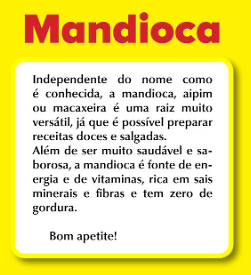
\includegraphics[width=2.61458in,height=2.86458in]{./imgSAEB_8_POR/media/image26.png}
% \caption{Texto Descrição gerada automaticamente}
\end{figure}

\fonte{CARQUEIJÓ, Joaquim. \emph{Arte da cozinha}, São Paulo, n.~03.} 

\num{9} Tipo de variação linguística:
\_\_\_\_\_\_\_\_\_\_\_\_\_\_\_\_\_\_\_\_\_\_\_\_\_\_\_\_\_\_\_\_\_ \rosa{geográfica}

Fator de influência:
\_\_\_\_\_\_\_\_\_\_\_\_\_\_\_\_\_\_\_\_\_\_\_\_\_\_\_\_\_\_\_\_\_\_\_\_\_\_ \rosa{região do falante}

\begin{quote}
A entrevista é o momento de comunicar quem você é, o que sabe fazer,
suas experiências anteriores e planos para o futuro. É nessa hora que
muita gente pisa na bola.

Para não chegar despreparado ao que pode ser o seu primeiro passo rumo a
uma carreira de sucesso, o segredo é estudar um bocado e seguir algumas
regras para mandar bem na entrevista. Descubra a seguir!

1. {[}...{]}

\textbf{Cuidado com a linguagem}

Ter um vocabulário adequado é importante para passar uma boa impressão
ao entrevistador. Por isso, evite a todo custo falar gírias, palavrões e
expressões chulas. Não que você precise ser excessivamente formal, ou
tenha que usar palavras difíceis. Basta ser simples e direto.
\end{quote}

\fonte{GUIA DA CARREIRA. Disponível em:
https://www.guiadacarreira.com.br/blog/cuidados-entrevista. Acesso em:
18 mar. 2023 (fragmento).}

Tipo de variação linguística:
\_\_\_\_\_\_\_\_\_\_\_\_\_\_\_\_\_\_\_\_\_\_\_\_\_\_\_\_\_\_\_\_\_ \rosa{situacional}

Fator de influência:
\_\_\_\_\_\_\_\_\_\_\_\_\_\_\_\_\_\_\_\_\_\_\_\_\_\_\_\_\_\_\_\_\_\_\_\_\_\_ \rosa{contexto comunicativo}

\section{Treino}

\num{0} Leia esta postagem do Tribunal Regional Eleitoral.

\begin{figure}
\centering

\includegraphics[width=5.26042in,height=1.47161in]{./imgSAEB_8_POR/media/image27.png}
% \caption{Interface gráfica do usuário, Texto, Aplicativo Descrição
% gerada automaticamente}
\end{figure}

Avalie a adequação da linguagem ao público-alvo da publicação.

\reduline{O público-alvo da publicação são os jovens, conhecidos por sua linguagem
característica permeada por gírias e expressões informais que
transgridem a norma-padrão, o que se identifica no texto da publicação.
Portanto, na tentativa de dialogar com esse público, a linguagem está
adequada.\hfill}
\linhas{6}

\num{1}

\begin{quote}\textbf{POPline}: Quando vocês {[}Nando Reis e Pitty{]} tiveram a ideia
de sair em turnê juntos? Foi papo de empresário ou partiu de vocês?

\textbf{Nando}: Então, na verdade não foi um papo de empresário coisa
nenhuma, foi uma ideia nossa. Começou há um ano e meio. Ela publicou um
vídeo dela cantando ``Relicário''. Eu fiquei super emocionado. Começamos
a conversar. Eu fiz um convite pra fazer o dueto {[}``Um tiro no
coração''{]} e imediatamente ela topou, mas falou ``eu quero mais''. E
daí pintou a ideia de fazer a turnê em que estamos trabalhando há um ano
e tanto.
\end{quote}
\fonte{Disponível em:
\url{https://portalpopline.com.br/entrevista-simbiose-pitty-nando-reis-nova-turne/.Acesso em: 18 mar. 2023 (fragmento adaptado).}}

Dois registros de variação linguística que influenciam o nível da
formalidade da entrevista são demonstrados em

\begin{escolha}
\item ``papo de empresário'' e ``pintou a ideia''.

\item ``Começamos a conversar'' e ``eu quero mais''.

\item ``Ela publicou um vídeo'' e ``foi uma ideia nossa''.

\item ``Um tiro no coração'' e ``Começou há um ano e meio''.
\end{escolha}

\num{2}

\textbf{Conexão}

\begin{quote}
Regido por esse despretensioso fluxo de ideias, me sinto tentado a fazer
uma parada. Até aqui me fiz tantas perguntas... Mas será que você,
leitor, é um jovem em busca de referências? Ou será que você é como eu
quando adolescente, que queria bater um papo sobre as identidades em
formação, mas sem um viés acadêmico? Só um papo que trouxesse conforto e
em que eu pudesse me espelhar... Quando, neste livro, eu sou você? Onde
nos encontramos? Em nossas semelhanças ou em nossas discordâncias?
\end{quote}
\fonte{RAMOS, Lázaro. \emph{Na minha pele}. 1.ed. Rio de Janeiro: Objetiva,
2017 (fragmento).}

A composição do texto privilegia o emprego de linguagem

\begin{escolha}
\item informal, visando interagir com o leitor.

\item culta, visando exibir domínio para o leitor.

\item formal, visando adequar-se ao público intelectual.

\item coloquial, visando atingir o leitor menos escolarizado.
\end{escolha}

\num{3}

\textbf{Mudança}

\begin{quote}
Levantei as 6 hóras preparando as roupas, fazendo trouxas para zarpar da
favela. Fiz o café e fui comprar pão, pedi ao Chico para atender-me logo
porque eu ia mudar.

-- Para onde?

-- Vou ressidir em Osasco.

Ele serviu logo, paguei e sai correndo.

Estava preparando os trastes quando chegou o senhor Paulino de Moura
dono da livraria Boulevard. Vêio convidar-me para eu ir na sua livraria
autografar os meus livros.

Eu disse-lhe que irei depois que agêitar a vida dos meus filhos porque,
quando eu os deixo na favela os favelados maltrata-os. {[}...{]}
\end{quote}
\fonte{JESUS, Carolina Maria de. \emph{Casa de alvenaria, volume 1}: Osasco.
1.ed. São Paulo: Companhia das Letras, 2021 (fragmento).}

O texto é um trecho do diário de Maria Carolina de Jesus publicado num
livro. Os acentos gráficos em ``hóras'', ``vêio'' e ``agêitar'' revelam
que sua escrita é fortemente influenciada pela

\begin{escolha}
\item idade.

\item escolaridade.

\item regionalidade.

\item informalidade.
\end{escolha}

\section{Referências}

ALMEIDA, L. de. \textbf{Análise semântica de operadores argumentativos
em textos publicitários}. 2001. 187 f.~Dissertação (Mestrado em Estudos
Linguísticos). Programa de PósGraduação em Estudos Linguísticos,
Instituto de Letras e Linguística, Universidade Federal de Uberlândia,
2001.

CEGALLA, Domingos Paschoal. \textbf{Novíssima gramática da língua
portuguesa}. 48. ed.~São Paulo: IBEP, 2009.

CHALHUB, Samira. \textbf{Funções da linguagem}. 11 ed.~São Paulo: Ática,
2000.

MARCUSCHI, Luiz Antônio. Gêneros textuais: definição e funcionalidade.
In: DIONISIO, Angela Paiva; MACHADO, Anna Rachel; BEZERRA, Maria
Auxiliadora (Org.). \textbf{Gêneros textuais \& ensino}. São Paulo:
Parábola, 2010. p.~23.

PORSCHE, Sandra Cristina. et al.~\textbf{O gênero verbete no ensino}.
Simpósio Internacional de Gêneros Textuais. Disponível em:
\textless{}\url{https://www.ucs.br/ucs/extensao/agenda/eventos/vsiget/portugues/anais/arquivos/o_genero_verbete_no_ensino.pdf}\textgreater.
Acessado em: 03/07/2018.

SARMENTO, Leila Luar: TUFANO: Douglas.~\textbf{Literatura, Gramática e
Produção de Texto}. São Paulo: Moderna, 2001.
